\documentclass[8pt]{report}
\usepackage{graphicx}
\parindent=0in
\textwidth=6.7in 
\textheight=9.5in
\setlength{\oddsidemargin}{-0.10in}
\setlength{\evensidemargin}{-0.10in}
\setlength{\topmargin}{-0.8in}
\setlength{\unitlength}{0.5in}
\pagestyle{empty}

\begin{document}

\begin{center}
{An\'alisis Estad\'stico de Datos (Examen Argumentativo)}
\end{center}

Nombre: \underline{\hspace*{.2in}}
Ana Sofía López
\underline{\hspace*{.2in}} \quad Matr\'icula:\underline{\hspace*{.2in}}
A0000001
\underline{\hspace*{.2in}} \\

{\bf Instrucciones:} Muestra c\'omo obtienes tu respuesta. Puedes usar Excel 
o Minitab para tus cálculos de probabilidades o 
percentiles, pero no uses otros archivos o hagas uso de la IA. Respeta el 
c\'odigo de \'etica del curso y del Tecnol\'ogico 
de Monterrey.


\begin{enumerate}

\item (16 pts) Una empresa que fabrica l\'aminas de aluminio 
para la industria aeron\'autica necesita asegurar que el espesor de sus l\'aminas 
cumple con las especificaciones de $2.50 \pm 0.10$ mm. Se ha implementado una nueva 
maquinaria y se desea monitorear el espesor de las l\'aminas. Para ello, se han 
tomado muestras de tama\~no 4 cada hora y se gener\'o el diagrama que se muestra 
abajo. Calcula los l\'imites de control para el espesor de las láminas.
\begin{figure}[h!]
\centering
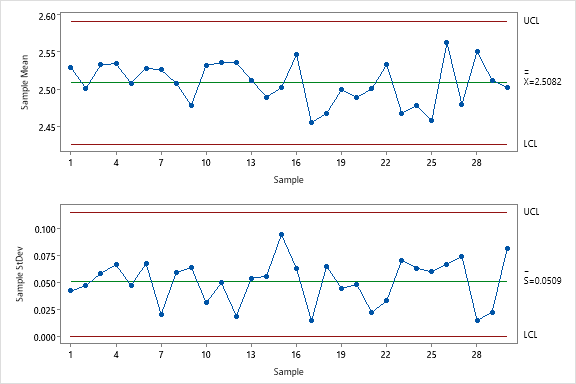
\includegraphics[width=0.5\textwidth]{Xbar_S_Paper.png}
\end{figure}


\item (14 pts) Una empresa que fabrica l\'aminas de aluminio para 
la industria aeron\'autica necesita asegurar que el espesor de sus l\'aminas cumple 
con las especificaciones de $2.50 \pm 0.10$ mm. Se ha implementado una nueva maquinaria 
y se desea monitorear el espesor de las l\'aminas. Para ello, se han tomado muestras 
de tama\~no 4 cada hora y se gener\'o el diagrama que se muestra abajo.
Calcula la probabilidad de que espesor de las láminas sea mayor 2.51 mm.
\begin{figure}[h!]
\centering
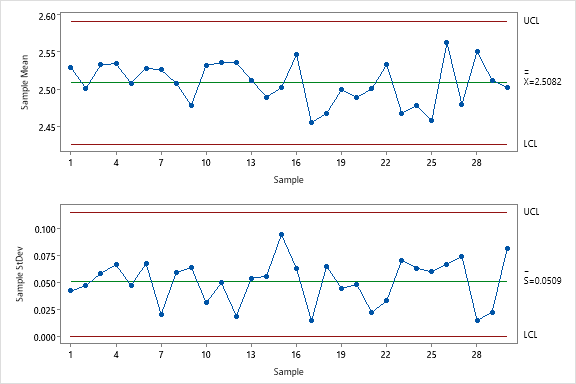
\includegraphics[width=0.5\textwidth]{Xbar_S_Paper.png}
\end{figure}


\item (14 pts) Una m\'aquina de inyecci\'on de pl\'astico 
produce piezas de precisi\'on. Se ha determinado que la probabilidad de que una 
pieza tenga una rebaba fuera de tolerancia es de $0.05$. Durante una auditor\'a 
de calidad, un inspector toma una muestra aleatoria de $n = 14$ piezas de la 
l\'inea de producci\'on. ¿Cu\'al es la probabilidad de que el inspector 
encuentre exactamente 3 piezas defectuosas en esa muestra?

\item (14 pts) En una l\'inea de producci\'on de ejes para 
motores, el di\'ametro es una caracter\'istica crítica para el ensamblaje adecuado. 
Las especificaciones del di\'ametro son $50.00 \pm 0.60$ mm. Se mide el di\'ametro 
de un eje cada 30 minutos. Despu\'es de 15 horas de mediciones, se obtuvo el 
gr\'afico IMR con un promedio m\'ovil de orden 2 que se muestra abajo.
¿Es el proceso es capaz de cumplir con las especificaciones? Argumente.
\begin{figure}[h!]
\centering
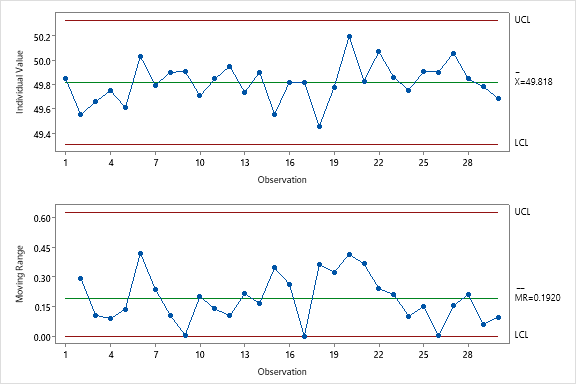
\includegraphics[width=0.5\textwidth]{IMR_Paper.png}
\end{figure}


\item (14 pts) Una empresa que fabrica tarjetas de circuitos 
impresos desea evaluar si la implementaci\'on de un nuevo sistema de ensamblaje 
ha reducido el n\'umero de disconformidades. Se tomaron 47 mediciones, antes y 
después del cambio, para analizar los efectos.
\begin{center}
\begin{tabular}{|l|c|c|}
\hline
 & Antes & Despu\'es \\ 
\hline
Media muestral & 3.60 & 3.54 \\ 
\hline
Desviaci\'on est\'andar muestral & 1.09 & 1.62 \\ 
\hline
\end{tabular}
\end{center}
¿Existe suficiente evidencia para concluir que el número medio de 
disconformidades ha disminuido despu\'es del cambio? Argumente.


\item (14 pts) Una empresa que fabrica l\'aminas de aluminio para 
la industria aeron\'autica necesita asegurar que el espesor de sus l\'aminas cumple 
con las especificaciones de $2.50 \pm 0.10$ mm. Se ha implementado una nueva maquinaria 
y se desea monitorear el espesor de las l\'aminas. Para ello, se han tomado muestras 
de tama\~no 4 cada hora y se gener\'o el diagrama que se muestra abajo.
Calcula los l\'imites de control para la {\bf variabilidad} del 
espesor de las láminas.
\begin{figure}[h!]
\centering
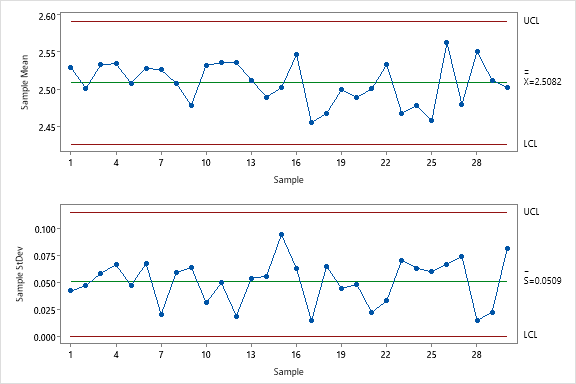
\includegraphics[width=0.5\textwidth]{Xbar_S_Paper.png}
\end{figure}


\item (14 pts) Una m\'aquina envasadora de detergente tiene 
una variabilidad natural con una desviaci\'on est\'andar de 8 ml, y la empresa 
debe garantizar que el 90.7\% de las botellas contengan al menos 500 ml para cumplir 
con la normativa de calidad. Determine a qu\'e valor promedio debe 
ajustarse la m\'aquina para que solo el 9.3\% de las botellas queden por debajo 
del contenido m\'inimo permitido.

\end{enumerate}

\newpage



\begin{center}
{An\'alisis Estad\'stico de Datos (Examen Argumentativo)}
\end{center}

Nombre: \underline{\hspace*{.2in}}
Carlos Eduardo García
\underline{\hspace*{.2in}} \quad Matr\'icula:\underline{\hspace*{.2in}}
A0000002
\underline{\hspace*{.2in}} \\

{\bf Instrucciones:} Muestra c\'omo obtienes tu respuesta. Puedes usar Excel 
o Minitab para tus cálculos de probabilidades o 
percentiles, pero no uses otros archivos o hagas uso de la IA. Respeta el 
c\'odigo de \'etica del curso y del Tecnol\'ogico 
de Monterrey.


\begin{enumerate}

\item (16 pts) Una empresa que fabrica l\'aminas de aluminio 
para la industria aeron\'autica necesita asegurar que el espesor de sus l\'aminas 
cumple con las especificaciones de $2.50 \pm 0.10$ mm. Se ha implementado una nueva 
maquinaria y se desea monitorear el espesor de las l\'aminas. Para ello, se han tomado 
muestras de tama\~no 5 cada hora y se gener\'o el diagrama que se muestra abajo.
Calcula los l\'imites de control para el espesor de las láminas.
\begin{figure}[h!]
\centering
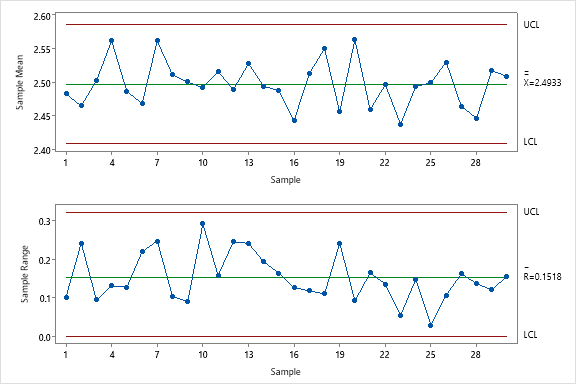
\includegraphics[width=0.5\textwidth]{Xbar_R_Paper.png}
\end{figure}


\item (14 pts) Una empresa que fabrica l\'aminas de aluminio para 
la industria aeron\'autica necesita asegurar que el espesor de sus l\'aminas cumple 
con las especificaciones de $2.50 \pm 0.10$ mm. Se ha implementado una nueva maquinaria 
y se desea monitorear el espesor de las l\'aminas. Para ello, se han tomado muestras 
de tama\~no 4 cada hora y se gener\'o el diagrama que se muestra abajo.
Calcula la probabilidad de que espesor de las láminas sea mayor 2.59 mm.
\begin{figure}[h!]
\centering
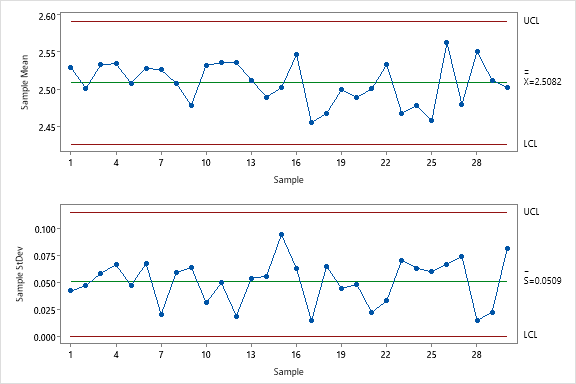
\includegraphics[width=0.5\textwidth]{Xbar_S_Paper.png}
\end{figure}


\item (14 pts) Una m\'aquina de inyecci\'on de pl\'astico 
produce piezas de precisi\'on. Se ha determinado que la probabilidad de que una 
pieza tenga una rebaba fuera de tolerancia es de $0.05$. Durante una auditor\'a 
de calidad, un inspector toma una muestra aleatoria de $n = 15$ piezas de la 
l\'inea de producci\'on. ¿Cu\'al es la probabilidad de que el inspector 
encuentre exactamente 4 piezas defectuosas en esa muestra?

\item (14 pts) En una l\'inea de producci\'on de ejes para 
motores, el di\'ametro es una caracter\'istica crítica para el ensamblaje adecuado. 
Las especificaciones del di\'ametro son $50.00 \pm 0.60$ mm. Se mide el di\'ametro 
de un eje cada 30 minutos. Despu\'es de 15 horas de mediciones, se obtuvo el 
gr\'afico IMR con un promedio m\'ovil de orden 2 que se muestra abajo.
¿Es el proceso es capaz de cumplir con las especificaciones? Argumente.
\begin{figure}[h!]
\centering
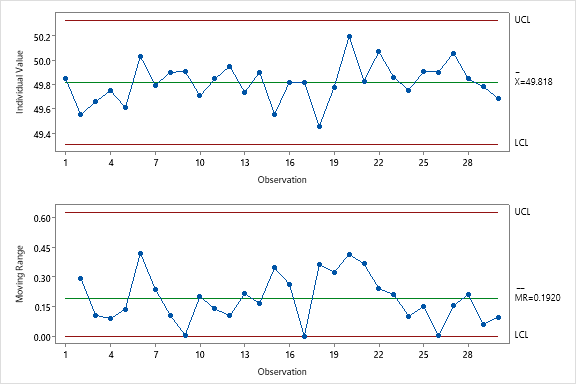
\includegraphics[width=0.5\textwidth]{IMR_Paper.png}
\end{figure}


\item (14 pts) Una empresa que fabrica tarjetas de circuitos 
impresos desea evaluar si la implementaci\'on de un nuevo sistema de ensamblaje 
ha reducido el n\'umero de disconformidades. Se tomaron 37 mediciones, antes y 
después del cambio, para analizar los efectos.
\begin{center}
\begin{tabular}{|l|c|c|}
\hline
 & Antes & Despu\'es \\ 
\hline
Media muestral & 3.60 & 2.58 \\ 
\hline
Desviaci\'on est\'andar muestral & 1.09 & 1.62 \\ 
\hline
\end{tabular}
\end{center}
¿Existe suficiente evidencia para concluir que el número medio de 
disconformidades ha disminuido despu\'es del cambio? Argumente.


\item (14 pts) Una empresa que fabrica l\'aminas de aluminio para 
la industria aeron\'autica necesita asegurar que el espesor de sus l\'aminas cumple 
con las especificaciones de $2.50 \pm 0.10$ mm. Se ha implementado una nueva maquinaria 
y se desea monitorear el espesor de las l\'aminas. Para ello, se han tomado muestras 
de tama\~no 4 cada hora y se gener\'o el diagrama que se muestra abajo.
Calcula los l\'imites de control para la {\bf variabilidad} del 
espesor de las láminas.
\begin{figure}[h!]
\centering
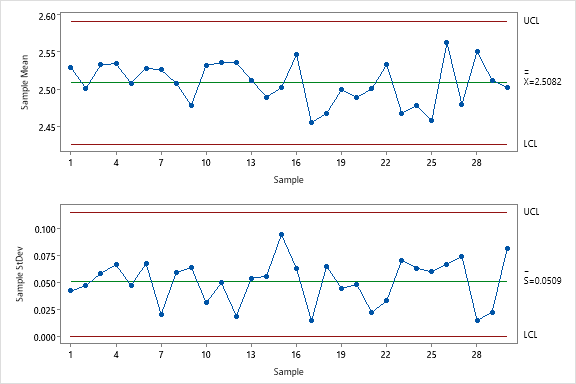
\includegraphics[width=0.5\textwidth]{Xbar_S_Paper.png}
\end{figure}


\item (14 pts) Una m\'aquina envasadora de detergente tiene 
una variabilidad natural con una desviaci\'on est\'andar de 8 ml, y la empresa 
debe garantizar que el 95.4\% de las botellas contengan al menos 500 ml para cumplir 
con la normativa de calidad. Determine a qu\'e valor promedio debe 
ajustarse la m\'aquina para que solo el 4.6\% de las botellas queden por debajo 
del contenido m\'inimo permitido.

\end{enumerate}

\newpage



\begin{center}
{An\'alisis Estad\'stico de Datos (Examen Argumentativo)}
\end{center}

Nombre: \underline{\hspace*{.2in}}
María Fernanda Ruiz
\underline{\hspace*{.2in}} \quad Matr\'icula:\underline{\hspace*{.2in}}
A0000003
\underline{\hspace*{.2in}} \\

{\bf Instrucciones:} Muestra c\'omo obtienes tu respuesta. Puedes usar Excel 
o Minitab para tus cálculos de probabilidades o 
percentiles, pero no uses otros archivos o hagas uso de la IA. Respeta el 
c\'odigo de \'etica del curso y del Tecnol\'ogico 
de Monterrey.


\begin{enumerate}

\item (16 pts) Una empresa que fabrica l\'aminas de aluminio 
para la industria aeron\'autica necesita asegurar que el espesor de sus l\'aminas 
cumple con las especificaciones de $2.50 \pm 0.10$ mm. Se ha implementado una nueva 
maquinaria y se desea monitorear el espesor de las l\'aminas. Para ello, se han 
tomado muestras de tama\~no 4 cada hora y se gener\'o el diagrama que se muestra 
abajo. Calcula los l\'imites de control para el espesor de las láminas.
\begin{figure}[h!]
\centering
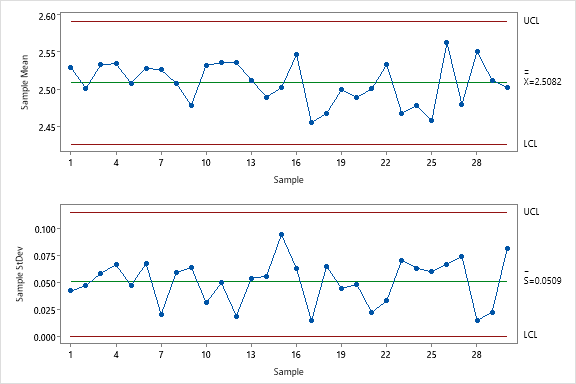
\includegraphics[width=0.5\textwidth]{Xbar_S_Paper.png}
\end{figure}


\item (14 pts) En una l\'inea de producci\'on de ejes para 
motores, el di\'ametro es una caracter\'istica crítica para el ensamblaje adecuado. 
Las especificaciones del di\'ametro son $50.00 \pm 0.50$ mm. Se mide el di\'ametro 
de un eje cada 30 minutos. Despu\'es de 15 horas de mediciones, se obtuvo el 
gr\'afico IMR con un promedio m\'ovil de orden 2 que se muestra abajo.
Calcula la probabilidad de que di\'ametro del eje se encuentre entre 49.8 mm y 
50.3 mm.
\begin{figure}[h!]
\centering
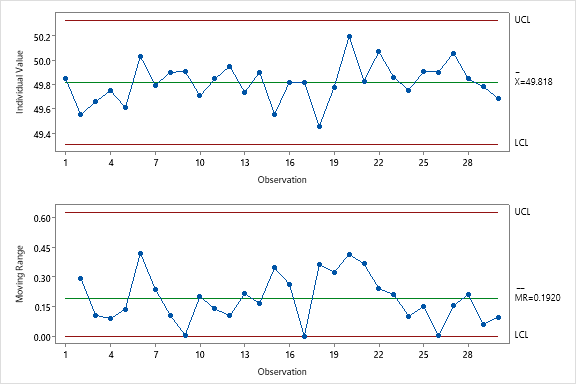
\includegraphics[width=0.5\textwidth]{IMR_Paper.png}
\end{figure}


\item (14 pts) Una m\'aquina de inyecci\'on de pl\'astico 
produce piezas de precisi\'on. Se ha determinado que la probabilidad de que una 
pieza tenga una rebaba fuera de tolerancia es de $0.05$. Durante una auditor\'a 
de calidad, un inspector toma una muestra aleatoria de $n = 15$ piezas de la 
l\'inea de producci\'on. ¿Cu\'al es la probabilidad de que el inspector 
encuentre exactamente 7 piezas defectuosas en esa muestra?

\item (14 pts) En una l\'inea de producci\'on de ejes para 
motores, el di\'ametro es una caracter\'istica crítica para el ensamblaje adecuado. 
Las especificaciones del di\'ametro son $50.00 \pm 0.60$ mm. Se mide el di\'ametro 
de un eje cada 30 minutos. Despu\'es de 15 horas de mediciones, se obtuvo el 
gr\'afico IMR con un promedio m\'ovil de orden 2 que se muestra abajo.
¿Es el proceso es capaz de cumplir con las especificaciones? Argumente.
\begin{figure}[h!]
\centering
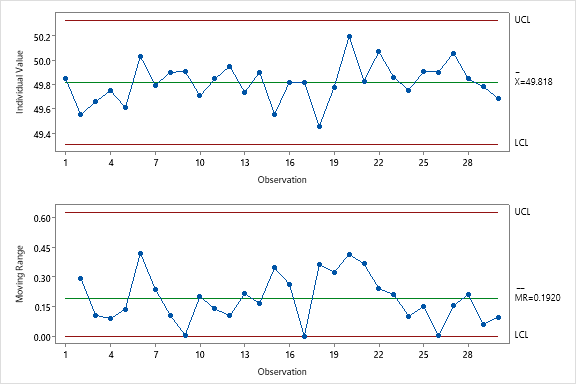
\includegraphics[width=0.5\textwidth]{IMR_Paper.png}
\end{figure}


\item (14 pts) Una empresa que fabrica tarjetas de circuitos 
impresos desea evaluar si la implementaci\'on de un nuevo sistema de ensamblaje 
ha reducido el n\'umero de disconformidades. Se tomaron 43 mediciones, antes y 
después del cambio, para analizar los efectos.
\begin{center}
\begin{tabular}{|l|c|c|}
\hline
 & Antes & Despu\'es \\ 
\hline
Media muestral & 3.60 & 3.00 \\ 
\hline
Desviaci\'on est\'andar muestral & 1.09 & 1.62 \\ 
\hline
\end{tabular}
\end{center}
¿Existe suficiente evidencia para concluir que el número medio de 
disconformidades ha disminuido despu\'es del cambio? Argumente.


\item (14 pts) Una empresa que fabrica l\'aminas de aluminio 
para la industria aeron\'autica necesita asegurar que el espesor de sus l\'aminas 
cumple con las especificaciones de $2.50 \pm 0.10$ mm. Se ha implementado una nueva 
maquinaria y se desea monitorear el espesor de las l\'aminas. Para ello, se han 
tomado muestras de tama\~no 5 cada hora y se gener\'o el diagrama que se muestra abajo.
Calcula los l\'imites de control para la {\bf variabilidad} del 
espesor de las láminas.
\begin{figure}[h!]
\centering
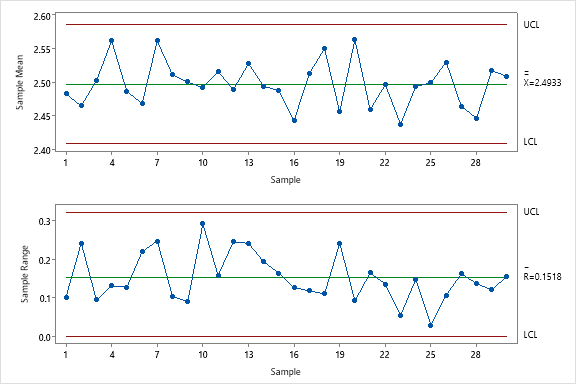
\includegraphics[width=0.5\textwidth]{Xbar_R_Paper.png}
\end{figure}


\item (14 pts) Una m\'aquina envasadora de detergente tiene 
una variabilidad natural con una desviaci\'on est\'andar de 8 ml, y la empresa 
debe garantizar que el 88.9\% de las botellas contengan al menos 500 ml para cumplir 
con la normativa de calidad. Determine a qu\'e valor promedio debe 
ajustarse la m\'aquina para que solo el 11.1\% de las botellas queden por debajo 
del contenido m\'inimo permitido.

\end{enumerate}

\newpage



\begin{center}
{An\'alisis Estad\'stico de Datos (Examen Argumentativo)}
\end{center}

Nombre: \underline{\hspace*{.2in}}
José Manuel Torres
\underline{\hspace*{.2in}} \quad Matr\'icula:\underline{\hspace*{.2in}}
A0000004
\underline{\hspace*{.2in}} \\

{\bf Instrucciones:} Muestra c\'omo obtienes tu respuesta. Puedes usar Excel 
o Minitab para tus cálculos de probabilidades o 
percentiles, pero no uses otros archivos o hagas uso de la IA. Respeta el 
c\'odigo de \'etica del curso y del Tecnol\'ogico 
de Monterrey.


\begin{enumerate}

\item (16 pts) Una empresa que fabrica l\'aminas de aluminio 
para la industria aeron\'autica necesita asegurar que el espesor de sus l\'aminas 
cumple con las especificaciones de $2.50 \pm 0.10$ mm. Se ha implementado una nueva 
maquinaria y se desea monitorear el espesor de las l\'aminas. Para ello, se han 
tomado muestras de tama\~no 4 cada hora y se gener\'o el diagrama que se muestra 
abajo. Calcula los l\'imites de control para el espesor de las láminas.
\begin{figure}[h!]
\centering
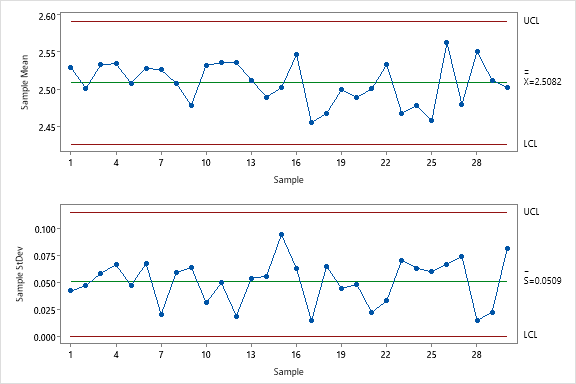
\includegraphics[width=0.5\textwidth]{Xbar_S_Paper.png}
\end{figure}


\item (14 pts) Una empresa que fabrica l\'aminas de aluminio para 
la industria aeron\'autica necesita asegurar que el espesor de sus l\'aminas cumple 
con las especificaciones de $2.50 \pm 0.10$ mm. Se ha implementado una nueva maquinaria 
y se desea monitorear el espesor de las l\'aminas. Para ello, se han tomado muestras 
de tama\~no 4 cada hora y se gener\'o el diagrama que se muestra abajo.
Calcula la probabilidad de que espesor de las láminas sea mayor 2.57 mm.
\begin{figure}[h!]
\centering
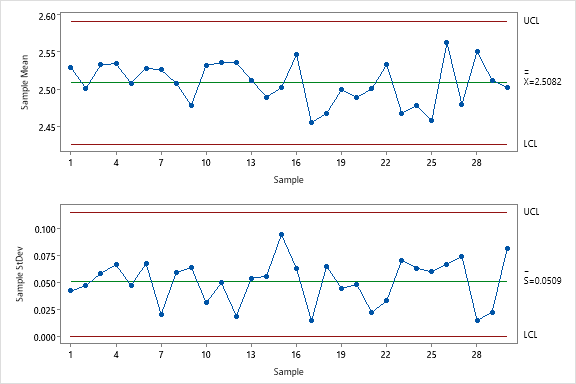
\includegraphics[width=0.5\textwidth]{Xbar_S_Paper.png}
\end{figure}


\item (14 pts) Una m\'aquina de inyecci\'on de pl\'astico 
produce piezas de precisi\'on. Se ha determinado que la probabilidad de que una 
pieza tenga una rebaba fuera de tolerancia es de $0.05$. Durante una auditor\'a 
de calidad, un inspector toma una muestra aleatoria de $n = 15$ piezas de la 
l\'inea de producci\'on. ¿Cu\'al es la probabilidad de que el inspector 
encuentre exactamente 4 piezas defectuosas en esa muestra?

\item (14 pts) En una l\'inea de producci\'on de ejes para 
motores, el di\'ametro es una caracter\'istica crítica para el ensamblaje adecuado. 
Las especificaciones del di\'ametro son $50.00 \pm 0.50$ mm. Se mide el di\'ametro 
de un eje cada 30 minutos. Despu\'es de 15 horas de mediciones, se obtuvo el 
gr\'afico IMR con un promedio m\'ovil de orden 2 que se muestra abajo.
¿Es el proceso es capaz de cumplir con las especificaciones? Argumente.
\begin{figure}[h!]
\centering
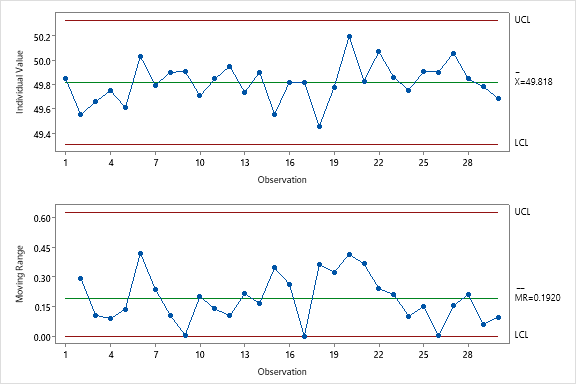
\includegraphics[width=0.5\textwidth]{IMR_Paper.png}
\end{figure}


\item (14 pts) Una empresa que fabrica tarjetas de circuitos 
impresos desea evaluar si la implementaci\'on de un nuevo sistema de ensamblaje 
ha reducido el n\'umero de disconformidades. Se tomaron 45 mediciones, antes y 
después del cambio, para analizar los efectos.
\begin{center}
\begin{tabular}{|l|c|c|}
\hline
 & Antes & Despu\'es \\ 
\hline
Media muestral & 3.60 & 2.54 \\ 
\hline
Desviaci\'on est\'andar muestral & 1.09 & 1.62 \\ 
\hline
\end{tabular}
\end{center}
¿Existe suficiente evidencia para concluir que el número medio de 
disconformidades ha disminuido despu\'es del cambio? Argumente.


\item (14 pts) Una empresa que fabrica l\'aminas de aluminio para 
la industria aeron\'autica necesita asegurar que el espesor de sus l\'aminas cumple 
con las especificaciones de $2.50 \pm 0.10$ mm. Se ha implementado una nueva maquinaria 
y se desea monitorear el espesor de las l\'aminas. Para ello, se han tomado muestras 
de tama\~no 4 cada hora y se gener\'o el diagrama que se muestra abajo.
Calcula los l\'imites de control para la {\bf variabilidad} del 
espesor de las láminas.
\begin{figure}[h!]
\centering
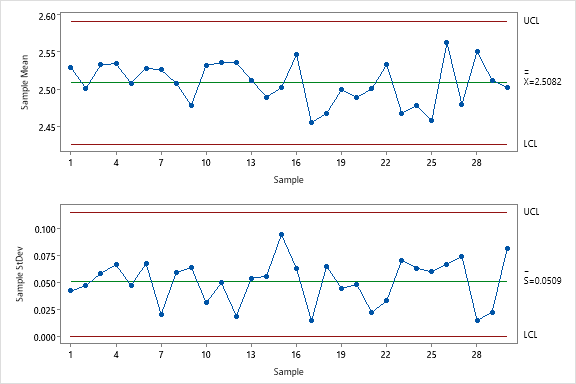
\includegraphics[width=0.5\textwidth]{Xbar_S_Paper.png}
\end{figure}


\item (14 pts) Una m\'aquina envasadora de detergente tiene 
una variabilidad natural con una desviaci\'on est\'andar de 8 ml, y la empresa 
debe garantizar que el 88.7\% de las botellas contengan al menos 500 ml para cumplir 
con la normativa de calidad. Determine a qu\'e valor promedio debe 
ajustarse la m\'aquina para que solo el 11.3\% de las botellas queden por debajo 
del contenido m\'inimo permitido.

\end{enumerate}

\newpage



\begin{center}
{An\'alisis Estad\'stico de Datos (Examen Argumentativo)}
\end{center}

Nombre: \underline{\hspace*{.2in}}
Daniela Hernández
\underline{\hspace*{.2in}} \quad Matr\'icula:\underline{\hspace*{.2in}}
A0000005
\underline{\hspace*{.2in}} \\

{\bf Instrucciones:} Muestra c\'omo obtienes tu respuesta. Puedes usar Excel 
o Minitab para tus cálculos de probabilidades o 
percentiles, pero no uses otros archivos o hagas uso de la IA. Respeta el 
c\'odigo de \'etica del curso y del Tecnol\'ogico 
de Monterrey.


\begin{enumerate}

\item (16 pts) Una empresa que fabrica l\'aminas de aluminio 
para la industria aeron\'autica necesita asegurar que el espesor de sus l\'aminas 
cumple con las especificaciones de $2.50 \pm 0.10$ mm. Se ha implementado una nueva 
maquinaria y se desea monitorear el espesor de las l\'aminas. Para ello, se han tomado 
muestras de tama\~no 5 cada hora y se gener\'o el diagrama que se muestra abajo.
Calcula los l\'imites de control para el espesor de las láminas.
\begin{figure}[h!]
\centering
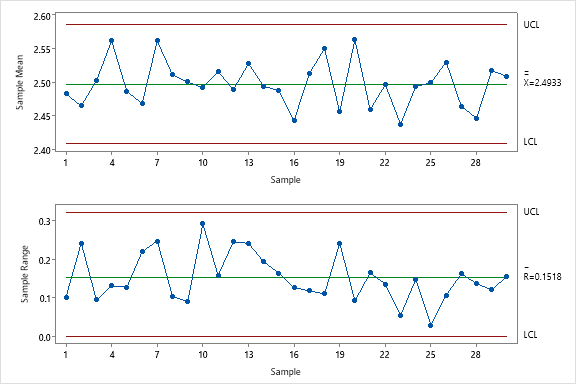
\includegraphics[width=0.5\textwidth]{Xbar_R_Paper.png}
\end{figure}


\item (14 pts) Una empresa que fabrica l\'aminas de aluminio para 
la industria aeron\'autica necesita asegurar que el espesor de sus l\'aminas cumple 
con las especificaciones de $2.50 \pm 0.10$ mm. Se ha implementado una nueva maquinaria 
y se desea monitorear el espesor de las l\'aminas. Para ello, se han tomado muestras 
de tama\~no 4 cada hora y se gener\'o el diagrama que se muestra abajo.
Calcula la probabilidad de que espesor de las láminas sea mayor 2.56 mm.
\begin{figure}[h!]
\centering
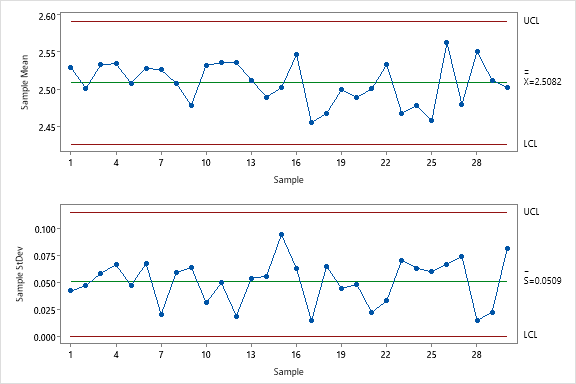
\includegraphics[width=0.5\textwidth]{Xbar_S_Paper.png}
\end{figure}


\item (14 pts) Una m\'aquina de inyecci\'on de pl\'astico 
produce piezas de precisi\'on. Se ha determinado que la probabilidad de que una 
pieza tenga una rebaba fuera de tolerancia es de $0.05$. Durante una auditor\'a 
de calidad, un inspector toma una muestra aleatoria de $n = 16$ piezas de la 
l\'inea de producci\'on. ¿Cu\'al es la probabilidad de que el inspector 
encuentre exactamente 5 piezas defectuosas en esa muestra?

\item (14 pts) En una l\'inea de producci\'on de ejes para 
motores, el di\'ametro es una caracter\'istica crítica para el ensamblaje adecuado. 
Las especificaciones del di\'ametro son $50.00 \pm 0.60$ mm. Se mide el di\'ametro 
de un eje cada 30 minutos. Despu\'es de 15 horas de mediciones, se obtuvo el 
gr\'afico IMR con un promedio m\'ovil de orden 2 que se muestra abajo.
¿Es el proceso es capaz de cumplir con las especificaciones? Argumente.
\begin{figure}[h!]
\centering
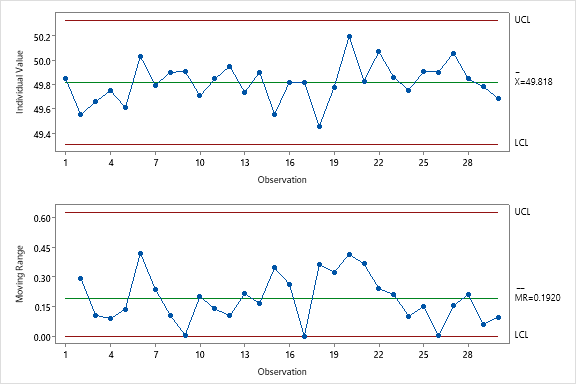
\includegraphics[width=0.5\textwidth]{IMR_Paper.png}
\end{figure}


\item (14 pts) Una empresa que fabrica tarjetas de circuitos 
impresos desea evaluar si la implementaci\'on de un nuevo sistema de ensamblaje 
ha reducido el n\'umero de disconformidades. Se tomaron 47 mediciones, antes y 
después del cambio, para analizar los efectos.
\begin{center}
\begin{tabular}{|l|c|c|}
\hline
 & Antes & Despu\'es \\ 
\hline
Media muestral & 3.60 & 3.00 \\ 
\hline
Desviaci\'on est\'andar muestral & 1.09 & 1.62 \\ 
\hline
\end{tabular}
\end{center}
Calcula un intervalo de confianza de 98\% para el número medio 
de disconformidades antes del cambio. Interprete su resultado.


\item (14 pts) Una empresa que fabrica l\'aminas de aluminio para 
la industria aeron\'autica necesita asegurar que el espesor de sus l\'aminas cumple 
con las especificaciones de $2.50 \pm 0.10$ mm. Se ha implementado una nueva maquinaria 
y se desea monitorear el espesor de las l\'aminas. Para ello, se han tomado muestras 
de tama\~no 4 cada hora y se gener\'o el diagrama que se muestra abajo.
Calcula los l\'imites de control para la {\bf variabilidad} del 
espesor de las láminas.
\begin{figure}[h!]
\centering
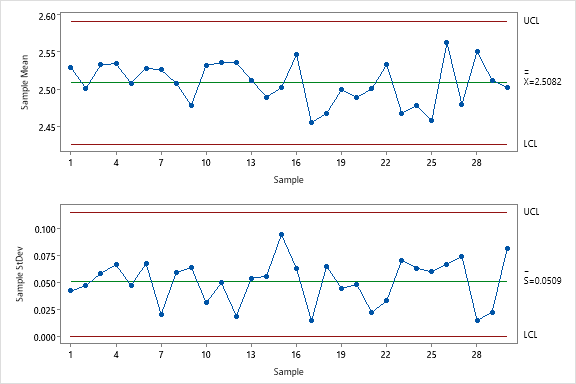
\includegraphics[width=0.5\textwidth]{Xbar_S_Paper.png}
\end{figure}


\item (14 pts) Una m\'aquina envasadora de detergente tiene 
una variabilidad natural con una desviaci\'on est\'andar de 8 ml, y la empresa 
debe garantizar que el 85.8\% de las botellas contengan al menos 500 ml para cumplir 
con la normativa de calidad. Determine a qu\'e valor promedio debe 
ajustarse la m\'aquina para que solo el 14.2\% de las botellas queden por debajo 
del contenido m\'inimo permitido.

\end{enumerate}

\newpage



\begin{center}
{An\'alisis Estad\'stico de Datos (Examen Argumentativo)}
\end{center}

Nombre: \underline{\hspace*{.2in}}
Luis Ángel Castro
\underline{\hspace*{.2in}} \quad Matr\'icula:\underline{\hspace*{.2in}}
A0000006
\underline{\hspace*{.2in}} \\

{\bf Instrucciones:} Muestra c\'omo obtienes tu respuesta. Puedes usar Excel 
o Minitab para tus cálculos de probabilidades o 
percentiles, pero no uses otros archivos o hagas uso de la IA. Respeta el 
c\'odigo de \'etica del curso y del Tecnol\'ogico 
de Monterrey.


\begin{enumerate}

\item (16 pts) Una empresa que fabrica l\'aminas de aluminio 
para la industria aeron\'autica necesita asegurar que el espesor de sus l\'aminas 
cumple con las especificaciones de $2.50 \pm 0.10$ mm. Se ha implementado una nueva 
maquinaria y se desea monitorear el espesor de las l\'aminas. Para ello, se han 
tomado muestras de tama\~no 4 cada hora y se gener\'o el diagrama que se muestra 
abajo. Calcula los l\'imites de control para el espesor de las láminas.
\begin{figure}[h!]
\centering
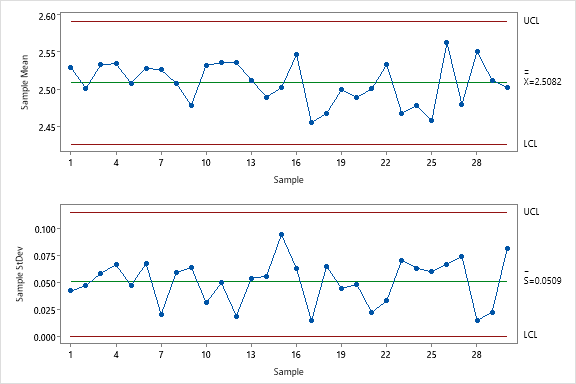
\includegraphics[width=0.5\textwidth]{Xbar_S_Paper.png}
\end{figure}


\item (14 pts) Una empresa que fabrica l\'aminas de aluminio para 
la industria aeron\'autica necesita asegurar que el espesor de sus l\'aminas cumple 
con las especificaciones de $2.50 \pm 0.10$ mm. Se ha implementado una nueva maquinaria 
y se desea monitorear el espesor de las l\'aminas. Para ello, se han tomado muestras 
de tama\~no 4 cada hora y se gener\'o el diagrama que se muestra abajo.
Calcula la probabilidad de que espesor de las láminas sea mayor 2.60 mm.
\begin{figure}[h!]
\centering
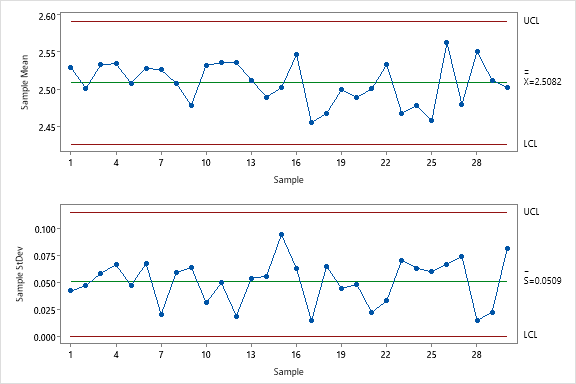
\includegraphics[width=0.5\textwidth]{Xbar_S_Paper.png}
\end{figure}


\item (14 pts) Una m\'aquina de inyecci\'on de pl\'astico 
produce piezas de precisi\'on. Se ha determinado que la probabilidad de que una 
pieza tenga una rebaba fuera de tolerancia es de $0.05$. Durante una auditor\'a 
de calidad, un inspector toma una muestra aleatoria de $n = 17$ piezas de la 
l\'inea de producci\'on. ¿Cu\'al es la probabilidad de que el inspector 
encuentre exactamente 6 piezas defectuosas en esa muestra?

\item (14 pts) En una l\'inea de producci\'on de ejes para 
motores, el di\'ametro es una caracter\'istica crítica para el ensamblaje adecuado. 
Las especificaciones del di\'ametro son $50.00 \pm 0.60$ mm. Se mide el di\'ametro 
de un eje cada 30 minutos. Despu\'es de 15 horas de mediciones, se obtuvo el 
gr\'afico IMR con un promedio m\'ovil de orden 2 que se muestra abajo.
¿Es el proceso es capaz de cumplir con las especificaciones? Argumente.
\begin{figure}[h!]
\centering
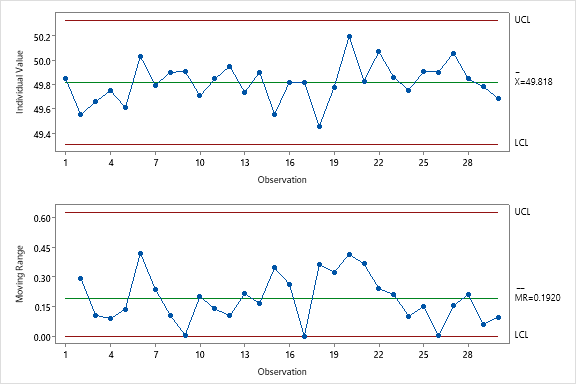
\includegraphics[width=0.5\textwidth]{IMR_Paper.png}
\end{figure}


\item (14 pts) Una empresa que fabrica tarjetas de circuitos 
impresos desea evaluar si la implementaci\'on de un nuevo sistema de ensamblaje 
ha reducido el n\'umero de disconformidades. Se tomaron 46 mediciones, antes y 
después del cambio, para analizar los efectos.
\begin{center}
\begin{tabular}{|l|c|c|}
\hline
 & Antes & Despu\'es \\ 
\hline
Media muestral & 3.60 & 3.46 \\ 
\hline
Desviaci\'on est\'andar muestral & 1.09 & 1.62 \\ 
\hline
\end{tabular}
\end{center}
¿Existe suficiente evidencia para concluir que el número medio de 
disconformidades ha disminuido despu\'es del cambio? Argumente.


\item (14 pts) Una empresa que fabrica l\'aminas de aluminio para 
la industria aeron\'autica necesita asegurar que el espesor de sus l\'aminas cumple 
con las especificaciones de $2.50 \pm 0.10$ mm. Se ha implementado una nueva maquinaria 
y se desea monitorear el espesor de las l\'aminas. Para ello, se han tomado muestras 
de tama\~no 4 cada hora y se gener\'o el diagrama que se muestra abajo.
Calcula los l\'imites de control para la {\bf variabilidad} del 
espesor de las láminas.
\begin{figure}[h!]
\centering
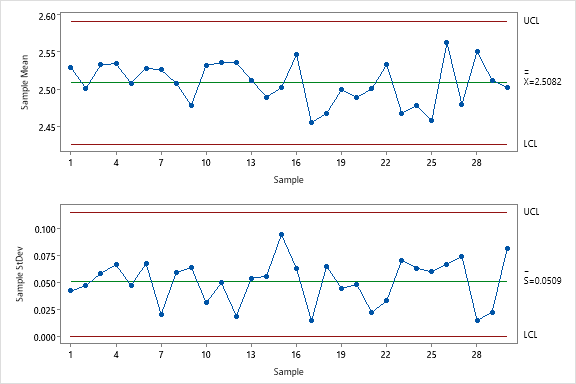
\includegraphics[width=0.5\textwidth]{Xbar_S_Paper.png}
\end{figure}


\item (14 pts) Una m\'aquina envasadora de detergente tiene 
una variabilidad natural con una desviaci\'on est\'andar de 8 ml, y la empresa 
debe garantizar que el 95.6\% de las botellas contengan al menos 500 ml para cumplir 
con la normativa de calidad. Determine a qu\'e valor promedio debe 
ajustarse la m\'aquina para que solo el 4.4\% de las botellas queden por debajo 
del contenido m\'inimo permitido.

\end{enumerate}

\newpage



\begin{center}
{An\'alisis Estad\'stico de Datos (Examen Argumentativo)}
\end{center}

Nombre: \underline{\hspace*{.2in}}
Valeria Mendoza
\underline{\hspace*{.2in}} \quad Matr\'icula:\underline{\hspace*{.2in}}
A0000007
\underline{\hspace*{.2in}} \\

{\bf Instrucciones:} Muestra c\'omo obtienes tu respuesta. Puedes usar Excel 
o Minitab para tus cálculos de probabilidades o 
percentiles, pero no uses otros archivos o hagas uso de la IA. Respeta el 
c\'odigo de \'etica del curso y del Tecnol\'ogico 
de Monterrey.


\begin{enumerate}

\item (16 pts) Una empresa que fabrica l\'aminas de aluminio 
para la industria aeron\'autica necesita asegurar que el espesor de sus l\'aminas 
cumple con las especificaciones de $2.50 \pm 0.10$ mm. Se ha implementado una nueva 
maquinaria y se desea monitorear el espesor de las l\'aminas. Para ello, se han 
tomado muestras de tama\~no 4 cada hora y se gener\'o el diagrama que se muestra 
abajo. Calcula los l\'imites de control para el espesor de las láminas.
\begin{figure}[h!]
\centering
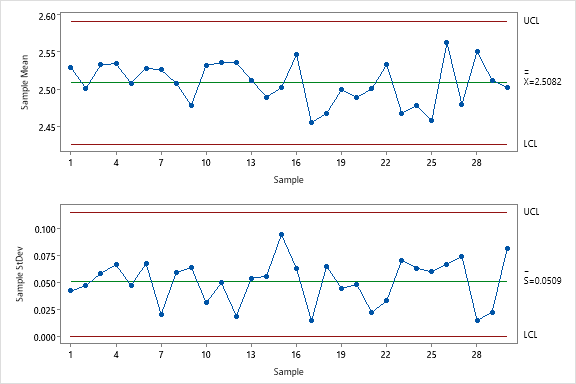
\includegraphics[width=0.5\textwidth]{Xbar_S_Paper.png}
\end{figure}


\item (14 pts) Una empresa que fabrica l\'aminas de aluminio para 
la industria aeron\'autica necesita asegurar que el espesor de sus l\'aminas cumple 
con las especificaciones de $2.50 \pm 0.10$ mm. Se ha implementado una nueva maquinaria 
y se desea monitorear el espesor de las l\'aminas. Para ello, se han tomado muestras 
de tama\~no 4 cada hora y se gener\'o el diagrama que se muestra abajo.
Calcula la probabilidad de que espesor de las láminas sea mayor 2.59 mm.
\begin{figure}[h!]
\centering
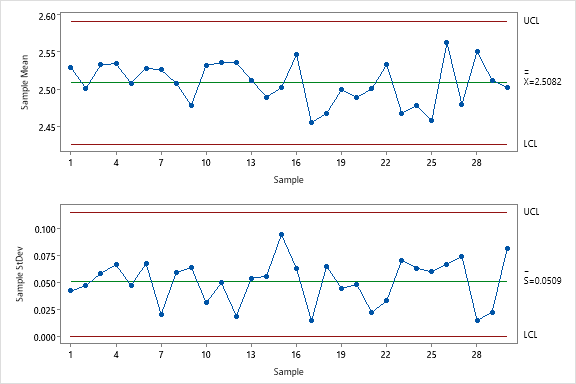
\includegraphics[width=0.5\textwidth]{Xbar_S_Paper.png}
\end{figure}


\item (14 pts) Una m\'aquina de inyecci\'on de pl\'astico 
produce piezas de precisi\'on. Se ha determinado que la probabilidad de que una 
pieza tenga una rebaba fuera de tolerancia es de $0.05$. Durante una auditor\'a 
de calidad, un inspector toma una muestra aleatoria de $n = 15$ piezas de la 
l\'inea de producci\'on. ¿Cu\'al es la probabilidad de que el inspector 
encuentre exactamente 4 piezas defectuosas en esa muestra?

\item (14 pts) Una empresa que fabrica l\'aminas de aluminio para 
la industria aeron\'autica necesita asegurar que el espesor de sus l\'aminas cumple 
con las especificaciones de $2.50 \pm 0.10$ mm. Se ha implementado una nueva maquinaria 
y se desea monitorear el espesor de las l\'aminas. Para ello, se han tomado muestras 
de tama\~no 4 cada hora y se gener\'o el diagrama que se muestra abajo.
¿Es el proceso es capaz de cumplir con las especificaciones? Argumente.
\begin{figure}[h!]
\centering
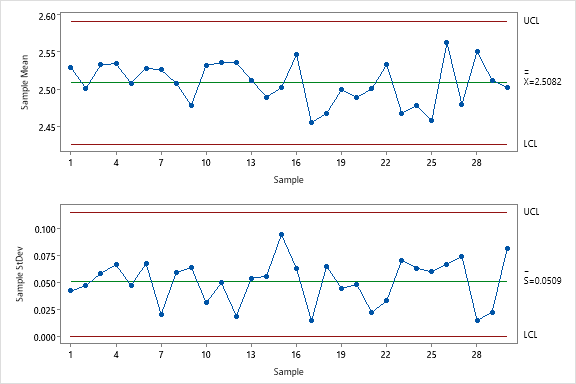
\includegraphics[width=0.5\textwidth]{Xbar_S_Paper.png}
\end{figure}


\item (14 pts) Una empresa que fabrica tarjetas de circuitos 
impresos desea evaluar si la implementaci\'on de un nuevo sistema de ensamblaje 
ha reducido el n\'umero de disconformidades. Se tomaron 39 mediciones, antes y 
después del cambio, para analizar los efectos.
\begin{center}
\begin{tabular}{|l|c|c|}
\hline
 & Antes & Despu\'es \\ 
\hline
Media muestral & 3.60 & 2.88 \\ 
\hline
Desviaci\'on est\'andar muestral & 1.09 & 1.62 \\ 
\hline
\end{tabular}
\end{center}
Calcula un intervalo de confianza de 90\% para el número medio 
de disconformidades antes del cambio. Interprete su resultado.


\item (14 pts) Una empresa que fabrica l\'aminas de aluminio 
para la industria aeron\'autica necesita asegurar que el espesor de sus l\'aminas 
cumple con las especificaciones de $2.50 \pm 0.10$ mm. Se ha implementado una nueva 
maquinaria y se desea monitorear el espesor de las l\'aminas. Para ello, se han 
tomado muestras de tama\~no 5 cada hora y se gener\'o el diagrama que se muestra abajo.
Calcula los l\'imites de control para la {\bf variabilidad} del 
espesor de las láminas.
\begin{figure}[h!]
\centering
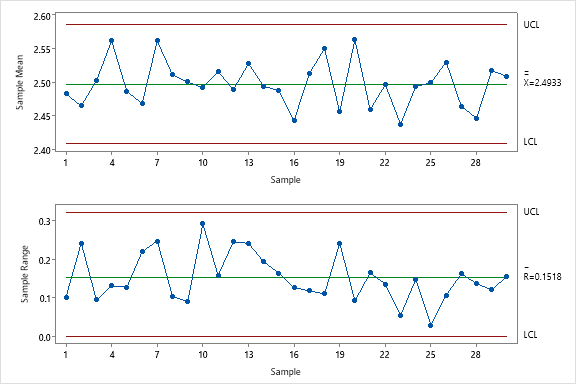
\includegraphics[width=0.5\textwidth]{Xbar_R_Paper.png}
\end{figure}


\item (14 pts) Una m\'aquina envasadora de detergente tiene 
una variabilidad natural con una desviaci\'on est\'andar de 8 ml, y la empresa 
debe garantizar que el 84.1\% de las botellas contengan al menos 500 ml para cumplir 
con la normativa de calidad. Determine a qu\'e valor promedio debe 
ajustarse la m\'aquina para que solo el 15.9\% de las botellas queden por debajo 
del contenido m\'inimo permitido.

\end{enumerate}

\newpage



\begin{center}
{An\'alisis Estad\'stico de Datos (Examen Argumentativo)}
\end{center}

Nombre: \underline{\hspace*{.2in}}
Diego Alejandro Vega
\underline{\hspace*{.2in}} \quad Matr\'icula:\underline{\hspace*{.2in}}
A0000008
\underline{\hspace*{.2in}} \\

{\bf Instrucciones:} Muestra c\'omo obtienes tu respuesta. Puedes usar Excel 
o Minitab para tus cálculos de probabilidades o 
percentiles, pero no uses otros archivos o hagas uso de la IA. Respeta el 
c\'odigo de \'etica del curso y del Tecnol\'ogico 
de Monterrey.


\begin{enumerate}

\item (16 pts) Una empresa que fabrica l\'aminas de aluminio 
para la industria aeron\'autica necesita asegurar que el espesor de sus l\'aminas 
cumple con las especificaciones de $2.50 \pm 0.10$ mm. Se ha implementado una nueva 
maquinaria y se desea monitorear el espesor de las l\'aminas. Para ello, se han 
tomado muestras de tama\~no 4 cada hora y se gener\'o el diagrama que se muestra 
abajo. Calcula los l\'imites de control para el espesor de las láminas.
\begin{figure}[h!]
\centering
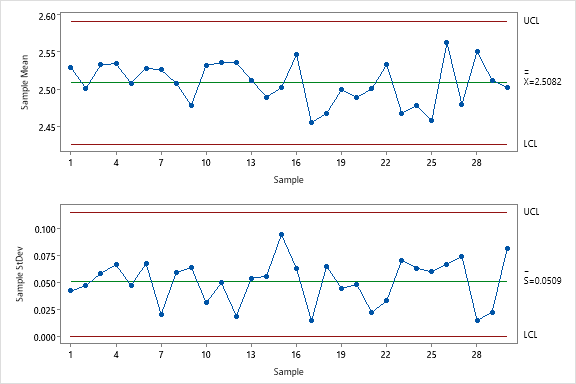
\includegraphics[width=0.5\textwidth]{Xbar_S_Paper.png}
\end{figure}


\item (14 pts) En una l\'inea de producci\'on de ejes para 
motores, el di\'ametro es una caracter\'istica crítica para el ensamblaje adecuado. 
Las especificaciones del di\'ametro son $50.00 \pm 0.50$ mm. Se mide el di\'ametro 
de un eje cada 30 minutos. Despu\'es de 15 horas de mediciones, se obtuvo el 
gr\'afico IMR con un promedio m\'ovil de orden 2 que se muestra abajo.
Calcula la probabilidad de que di\'ametro del eje se encuentre entre 49.7 mm y 
50.1 mm.
\begin{figure}[h!]
\centering
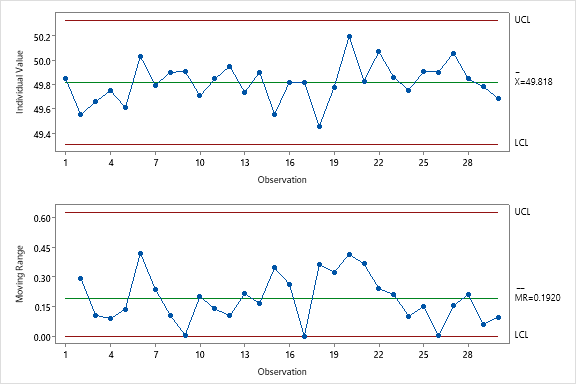
\includegraphics[width=0.5\textwidth]{IMR_Paper.png}
\end{figure}


\item (14 pts) Una m\'aquina de inyecci\'on de pl\'astico 
produce piezas de precisi\'on. Se ha determinado que la probabilidad de que una 
pieza tenga una rebaba fuera de tolerancia es de $0.05$. Durante una auditor\'a 
de calidad, un inspector toma una muestra aleatoria de $n = 15$ piezas de la 
l\'inea de producci\'on. ¿Cu\'al es la probabilidad de que el inspector 
encuentre exactamente 4 piezas defectuosas en esa muestra?

\item (14 pts) Una empresa que fabrica l\'aminas de aluminio para 
la industria aeron\'autica necesita asegurar que el espesor de sus l\'aminas cumple 
con las especificaciones de $2.50 \pm 0.10$ mm. Se ha implementado una nueva maquinaria 
y se desea monitorear el espesor de las l\'aminas. Para ello, se han tomado muestras 
de tama\~no 4 cada hora y se gener\'o el diagrama que se muestra abajo.
¿Es el proceso es capaz de cumplir con las especificaciones? Argumente.
\begin{figure}[h!]
\centering
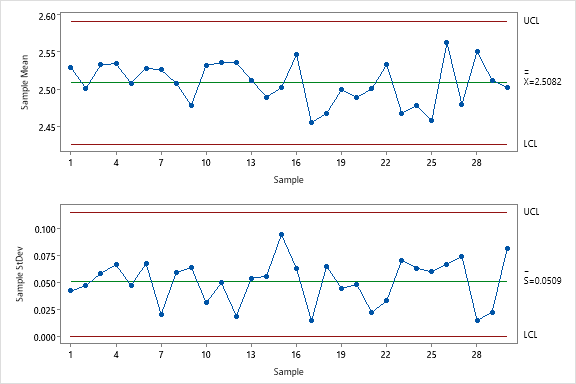
\includegraphics[width=0.5\textwidth]{Xbar_S_Paper.png}
\end{figure}


\item (14 pts) Una empresa que fabrica tarjetas de circuitos 
impresos desea evaluar si la implementaci\'on de un nuevo sistema de ensamblaje 
ha reducido el n\'umero de disconformidades. Se tomaron 45 mediciones, antes y 
después del cambio, para analizar los efectos.
\begin{center}
\begin{tabular}{|l|c|c|}
\hline
 & Antes & Despu\'es \\ 
\hline
Media muestral & 3.60 & 3.45 \\ 
\hline
Desviaci\'on est\'andar muestral & 1.09 & 1.62 \\ 
\hline
\end{tabular}
\end{center}
Calcula un intervalo de confianza de 92\% para el número medio 
de disconformidades antes del cambio. Interprete su resultado.


\item (14 pts) Una empresa que fabrica l\'aminas de aluminio 
para la industria aeron\'autica necesita asegurar que el espesor de sus l\'aminas 
cumple con las especificaciones de $2.50 \pm 0.10$ mm. Se ha implementado una nueva 
maquinaria y se desea monitorear el espesor de las l\'aminas. Para ello, se han 
tomado muestras de tama\~no 5 cada hora y se gener\'o el diagrama que se muestra abajo.
Calcula los l\'imites de control para la {\bf variabilidad} del 
espesor de las láminas.
\begin{figure}[h!]
\centering
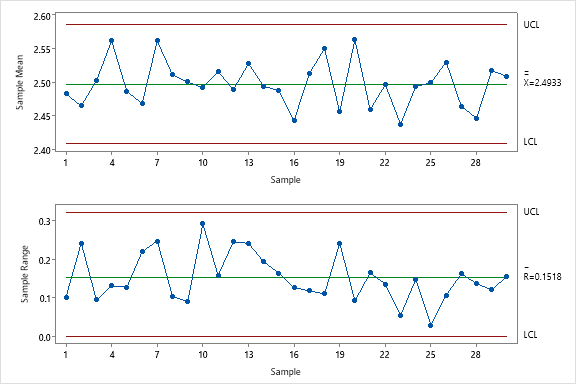
\includegraphics[width=0.5\textwidth]{Xbar_R_Paper.png}
\end{figure}


\item (14 pts) Una m\'aquina envasadora de detergente tiene 
una variabilidad natural con una desviaci\'on est\'andar de 8 ml, y la empresa 
debe garantizar que el 84.3\% de las botellas contengan al menos 500 ml para cumplir 
con la normativa de calidad. Determine a qu\'e valor promedio debe 
ajustarse la m\'aquina para que solo el 15.7\% de las botellas queden por debajo 
del contenido m\'inimo permitido.

\end{enumerate}

\newpage



\begin{center}
{An\'alisis Estad\'stico de Datos (Examen Argumentativo)}
\end{center}

Nombre: \underline{\hspace*{.2in}}
Fernanda Cárdenas
\underline{\hspace*{.2in}} \quad Matr\'icula:\underline{\hspace*{.2in}}
A0000009
\underline{\hspace*{.2in}} \\

{\bf Instrucciones:} Muestra c\'omo obtienes tu respuesta. Puedes usar Excel 
o Minitab para tus cálculos de probabilidades o 
percentiles, pero no uses otros archivos o hagas uso de la IA. Respeta el 
c\'odigo de \'etica del curso y del Tecnol\'ogico 
de Monterrey.


\begin{enumerate}

\item (16 pts) Una empresa que fabrica l\'aminas de aluminio 
para la industria aeron\'autica necesita asegurar que el espesor de sus l\'aminas 
cumple con las especificaciones de $2.50 \pm 0.10$ mm. Se ha implementado una nueva 
maquinaria y se desea monitorear el espesor de las l\'aminas. Para ello, se han 
tomado muestras de tama\~no 4 cada hora y se gener\'o el diagrama que se muestra 
abajo. Calcula los l\'imites de control para el espesor de las láminas.
\begin{figure}[h!]
\centering
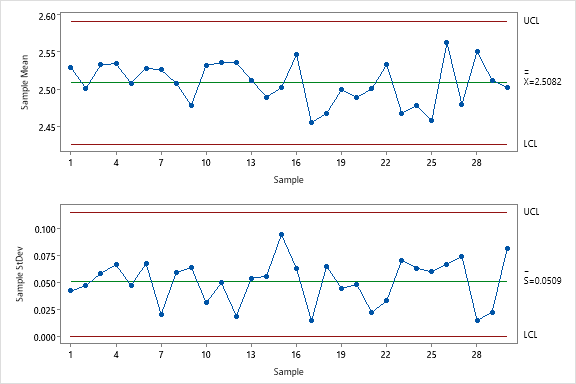
\includegraphics[width=0.5\textwidth]{Xbar_S_Paper.png}
\end{figure}


\item (14 pts) En una l\'inea de producci\'on de ejes para 
motores, el di\'ametro es una caracter\'istica crítica para el ensamblaje adecuado. 
Las especificaciones del di\'ametro son $50.00 \pm 0.50$ mm. Se mide el di\'ametro 
de un eje cada 30 minutos. Despu\'es de 15 horas de mediciones, se obtuvo el 
gr\'afico IMR con un promedio m\'ovil de orden 2 que se muestra abajo.
Calcula la probabilidad de que di\'ametro del eje se encuentre entre 49.6 mm y 
50.4 mm.
\begin{figure}[h!]
\centering
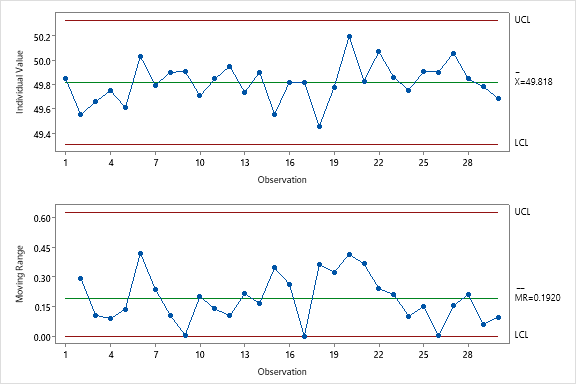
\includegraphics[width=0.5\textwidth]{IMR_Paper.png}
\end{figure}


\item (14 pts) Una m\'aquina de inyecci\'on de pl\'astico 
produce piezas de precisi\'on. Se ha determinado que la probabilidad de que una 
pieza tenga una rebaba fuera de tolerancia es de $0.05$. Durante una auditor\'a 
de calidad, un inspector toma una muestra aleatoria de $n = 13$ piezas de la 
l\'inea de producci\'on. ¿Cu\'al es la probabilidad de que el inspector 
encuentre exactamente 6 piezas defectuosas en esa muestra?

\item (14 pts) En una l\'inea de producci\'on de ejes para 
motores, el di\'ametro es una caracter\'istica crítica para el ensamblaje adecuado. 
Las especificaciones del di\'ametro son $50.00 \pm 0.60$ mm. Se mide el di\'ametro 
de un eje cada 30 minutos. Despu\'es de 15 horas de mediciones, se obtuvo el 
gr\'afico IMR con un promedio m\'ovil de orden 2 que se muestra abajo.
¿Es el proceso es capaz de cumplir con las especificaciones? Argumente.
\begin{figure}[h!]
\centering
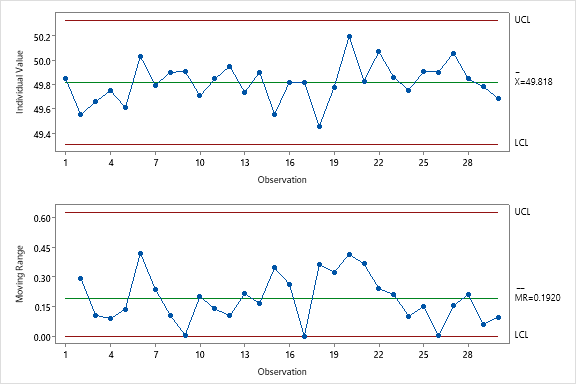
\includegraphics[width=0.5\textwidth]{IMR_Paper.png}
\end{figure}


\item (14 pts) Una empresa que fabrica tarjetas de circuitos 
impresos desea evaluar si la implementaci\'on de un nuevo sistema de ensamblaje 
ha reducido el n\'umero de disconformidades. Se tomaron 42 mediciones, antes y 
después del cambio, para analizar los efectos.
\begin{center}
\begin{tabular}{|l|c|c|}
\hline
 & Antes & Despu\'es \\ 
\hline
Media muestral & 3.60 & 2.93 \\ 
\hline
Desviaci\'on est\'andar muestral & 1.09 & 1.62 \\ 
\hline
\end{tabular}
\end{center}
Calcula un intervalo de confianza de 97\% para el número medio 
de disconformidades antes del cambio. Interprete su resultado.


\item (14 pts) Una empresa que fabrica l\'aminas de aluminio 
para la industria aeron\'autica necesita asegurar que el espesor de sus l\'aminas 
cumple con las especificaciones de $2.50 \pm 0.10$ mm. Se ha implementado una nueva 
maquinaria y se desea monitorear el espesor de las l\'aminas. Para ello, se han 
tomado muestras de tama\~no 5 cada hora y se gener\'o el diagrama que se muestra abajo.
Calcula los l\'imites de control para la {\bf variabilidad} del 
espesor de las láminas.
\begin{figure}[h!]
\centering
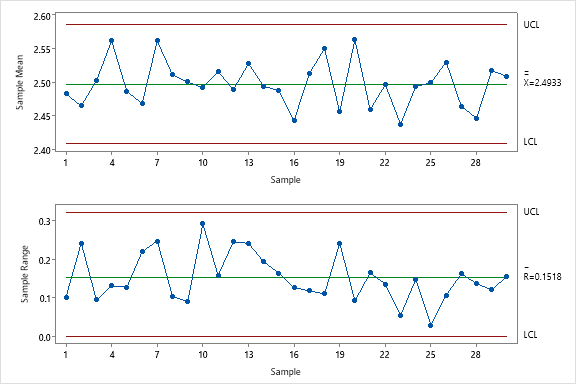
\includegraphics[width=0.5\textwidth]{Xbar_R_Paper.png}
\end{figure}


\item (14 pts) Una m\'aquina envasadora de detergente tiene 
una variabilidad natural con una desviaci\'on est\'andar de 8 ml, y la empresa 
debe garantizar que el 86.1\% de las botellas contengan al menos 500 ml para cumplir 
con la normativa de calidad. Determine a qu\'e valor promedio debe 
ajustarse la m\'aquina para que solo el 13.9\% de las botellas queden por debajo 
del contenido m\'inimo permitido.

\end{enumerate}

\newpage



\begin{center}
{An\'alisis Estad\'stico de Datos (Examen Argumentativo)}
\end{center}

Nombre: \underline{\hspace*{.2in}}
Miguel Ángel Ríos
\underline{\hspace*{.2in}} \quad Matr\'icula:\underline{\hspace*{.2in}}
A0000010
\underline{\hspace*{.2in}} \\

{\bf Instrucciones:} Muestra c\'omo obtienes tu respuesta. Puedes usar Excel 
o Minitab para tus cálculos de probabilidades o 
percentiles, pero no uses otros archivos o hagas uso de la IA. Respeta el 
c\'odigo de \'etica del curso y del Tecnol\'ogico 
de Monterrey.


\begin{enumerate}

\item (16 pts) Una empresa que fabrica l\'aminas de aluminio 
para la industria aeron\'autica necesita asegurar que el espesor de sus l\'aminas 
cumple con las especificaciones de $2.50 \pm 0.10$ mm. Se ha implementado una nueva 
maquinaria y se desea monitorear el espesor de las l\'aminas. Para ello, se han 
tomado muestras de tama\~no 4 cada hora y se gener\'o el diagrama que se muestra 
abajo. Calcula los l\'imites de control para el espesor de las láminas.
\begin{figure}[h!]
\centering
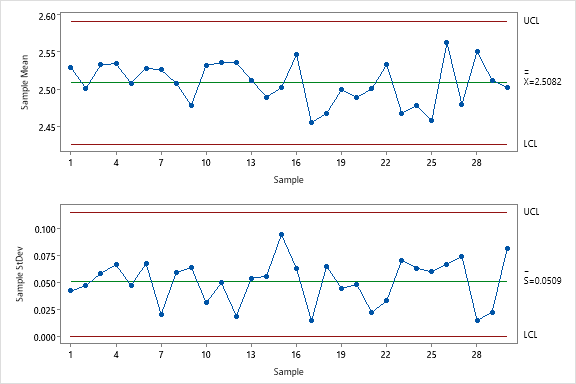
\includegraphics[width=0.5\textwidth]{Xbar_S_Paper.png}
\end{figure}


\item (14 pts) Una empresa que fabrica l\'aminas de aluminio para 
la industria aeron\'autica necesita asegurar que el espesor de sus l\'aminas cumple 
con las especificaciones de $2.50 \pm 0.10$ mm. Se ha implementado una nueva maquinaria 
y se desea monitorear el espesor de las l\'aminas. Para ello, se han tomado muestras 
de tama\~no 4 cada hora y se gener\'o el diagrama que se muestra abajo.
Calcula la probabilidad de que espesor de las láminas sea mayor 2.55 mm.
\begin{figure}[h!]
\centering
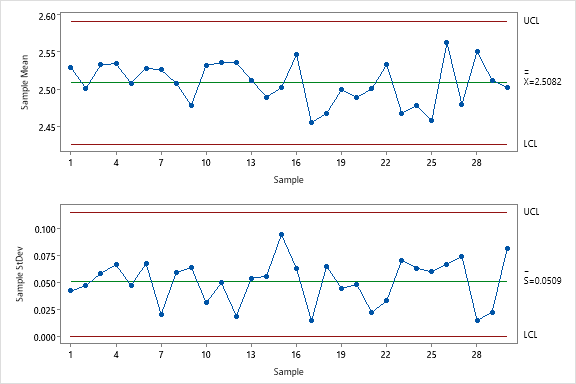
\includegraphics[width=0.5\textwidth]{Xbar_S_Paper.png}
\end{figure}


\item (14 pts) Una m\'aquina de inyecci\'on de pl\'astico 
produce piezas de precisi\'on. Se ha determinado que la probabilidad de que una 
pieza tenga una rebaba fuera de tolerancia es de $0.05$. Durante una auditor\'a 
de calidad, un inspector toma una muestra aleatoria de $n = 14$ piezas de la 
l\'inea de producci\'on. ¿Cu\'al es la probabilidad de que el inspector 
encuentre exactamente 6 piezas defectuosas en esa muestra?

\item (14 pts) En una l\'inea de producci\'on de ejes para 
motores, el di\'ametro es una caracter\'istica crítica para el ensamblaje adecuado. 
Las especificaciones del di\'ametro son $50.00 \pm 0.50$ mm. Se mide el di\'ametro 
de un eje cada 30 minutos. Despu\'es de 15 horas de mediciones, se obtuvo el 
gr\'afico IMR con un promedio m\'ovil de orden 2 que se muestra abajo.
¿Es el proceso es capaz de cumplir con las especificaciones? Argumente.
\begin{figure}[h!]
\centering
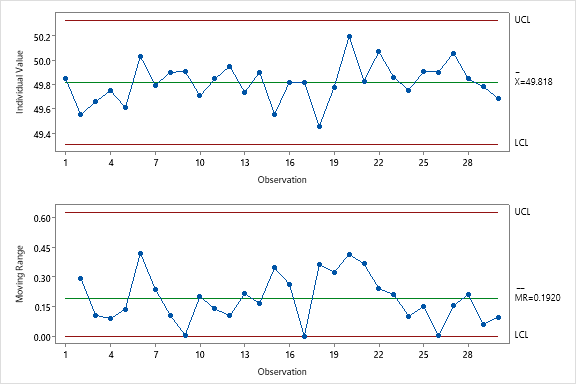
\includegraphics[width=0.5\textwidth]{IMR_Paper.png}
\end{figure}


\item (14 pts) Una empresa que fabrica tarjetas de circuitos 
impresos desea evaluar si la implementaci\'on de un nuevo sistema de ensamblaje 
ha reducido el n\'umero de disconformidades. Se tomaron 42 mediciones, antes y 
después del cambio, para analizar los efectos.
\begin{center}
\begin{tabular}{|l|c|c|}
\hline
 & Antes & Despu\'es \\ 
\hline
Media muestral & 3.60 & 2.96 \\ 
\hline
Desviaci\'on est\'andar muestral & 1.09 & 1.62 \\ 
\hline
\end{tabular}
\end{center}
Calcula un intervalo de confianza de 94\% para el número medio 
de disconformidades antes del cambio. Interprete su resultado.


\item (14 pts) Una empresa que fabrica l\'aminas de aluminio para 
la industria aeron\'autica necesita asegurar que el espesor de sus l\'aminas cumple 
con las especificaciones de $2.50 \pm 0.10$ mm. Se ha implementado una nueva maquinaria 
y se desea monitorear el espesor de las l\'aminas. Para ello, se han tomado muestras 
de tama\~no 4 cada hora y se gener\'o el diagrama que se muestra abajo.
Calcula los l\'imites de control para la {\bf variabilidad} del 
espesor de las láminas.
\begin{figure}[h!]
\centering
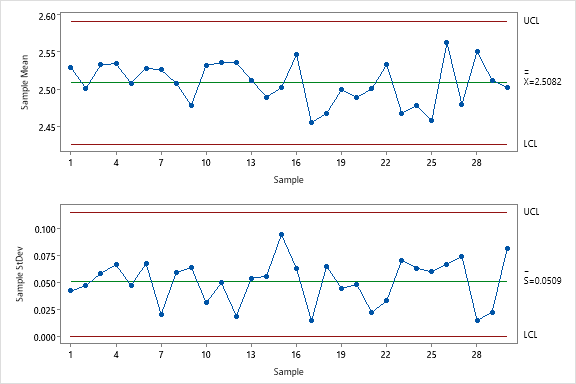
\includegraphics[width=0.5\textwidth]{Xbar_S_Paper.png}
\end{figure}


\item (14 pts) Una m\'aquina envasadora de detergente tiene 
una variabilidad natural con una desviaci\'on est\'andar de 8 ml, y la empresa 
debe garantizar que el 95.5\% de las botellas contengan al menos 500 ml para cumplir 
con la normativa de calidad. Determine a qu\'e valor promedio debe 
ajustarse la m\'aquina para que solo el 4.5\% de las botellas queden por debajo 
del contenido m\'inimo permitido.

\end{enumerate}

\newpage



\begin{center}
{An\'alisis Estad\'stico de Datos (Examen Argumentativo)}
\end{center}

Nombre: \underline{\hspace*{.2in}}
Andrea Martínez
\underline{\hspace*{.2in}} \quad Matr\'icula:\underline{\hspace*{.2in}}
A0000011
\underline{\hspace*{.2in}} \\

{\bf Instrucciones:} Muestra c\'omo obtienes tu respuesta. Puedes usar Excel 
o Minitab para tus cálculos de probabilidades o 
percentiles, pero no uses otros archivos o hagas uso de la IA. Respeta el 
c\'odigo de \'etica del curso y del Tecnol\'ogico 
de Monterrey.


\begin{enumerate}

\item (16 pts) En una l\'inea de producci\'on de ejes para 
motores, el di\'ametro es una caracter\'istica crítica para el ensamblaje adecuado. 
Las especificaciones del di\'ametro son $50.00 \pm 0.50$ mm. Se mide el di\'ametro 
de un eje cada 30 minutos. Despu\'es de 15 horas de mediciones, se obtuvo el 
gr\'afico IMR con un promedio m\'ovil de orden 2 que se muestra abajo. 
Calcula los l\'imites de control para el di\'ametro del eje.
\begin{figure}[h!]
\centering
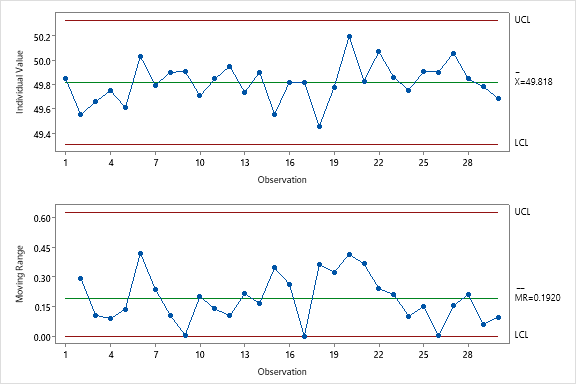
\includegraphics[width=0.5\textwidth]{IMR_Paper.png}
\end{figure}


\item (14 pts) Una empresa que fabrica l\'aminas de aluminio para 
la industria aeron\'autica necesita asegurar que el espesor de sus l\'aminas cumple 
con las especificaciones de $2.50 \pm 0.10$ mm. Se ha implementado una nueva maquinaria 
y se desea monitorear el espesor de las l\'aminas. Para ello, se han tomado muestras 
de tama\~no 4 cada hora y se gener\'o el diagrama que se muestra abajo.
Calcula la probabilidad de que espesor de las láminas sea mayor 2.52 mm.
\begin{figure}[h!]
\centering
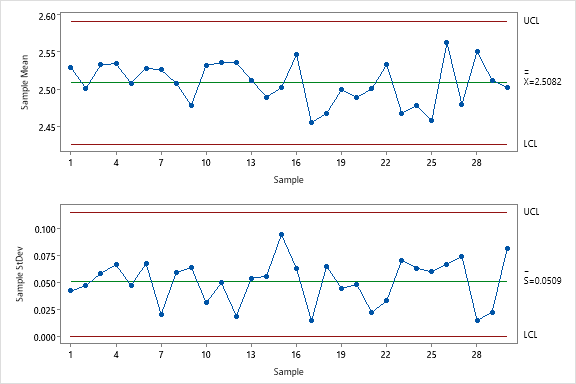
\includegraphics[width=0.5\textwidth]{Xbar_S_Paper.png}
\end{figure}


\item (14 pts) Una m\'aquina de inyecci\'on de pl\'astico 
produce piezas de precisi\'on. Se ha determinado que la probabilidad de que una 
pieza tenga una rebaba fuera de tolerancia es de $0.05$. Durante una auditor\'a 
de calidad, un inspector toma una muestra aleatoria de $n = 14$ piezas de la 
l\'inea de producci\'on. ¿Cu\'al es la probabilidad de que el inspector 
encuentre exactamente 6 piezas defectuosas en esa muestra?

\item (14 pts) Una empresa que fabrica l\'aminas de aluminio para 
la industria aeron\'autica necesita asegurar que el espesor de sus l\'aminas cumple 
con las especificaciones de $2.50 \pm 0.10$ mm. Se ha implementado una nueva maquinaria 
y se desea monitorear el espesor de las l\'aminas. Para ello, se han tomado muestras 
de tama\~no 4 cada hora y se gener\'o el diagrama que se muestra abajo.
¿Es el proceso es capaz de cumplir con las especificaciones? Argumente.
\begin{figure}[h!]
\centering
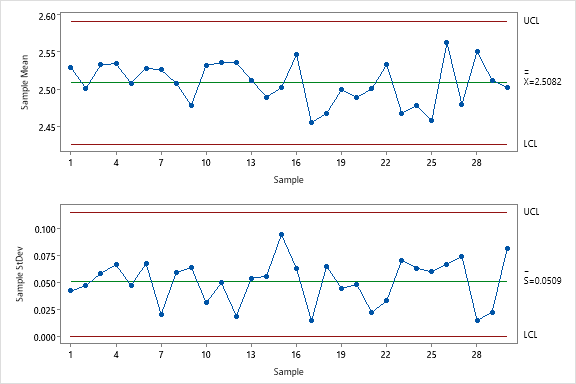
\includegraphics[width=0.5\textwidth]{Xbar_S_Paper.png}
\end{figure}


\item (14 pts) Una empresa que fabrica tarjetas de circuitos 
impresos desea evaluar si la implementaci\'on de un nuevo sistema de ensamblaje 
ha reducido el n\'umero de disconformidades. Se tomaron 48 mediciones, antes y 
después del cambio, para analizar los efectos.
\begin{center}
\begin{tabular}{|l|c|c|}
\hline
 & Antes & Despu\'es \\ 
\hline
Media muestral & 3.60 & 2.96 \\ 
\hline
Desviaci\'on est\'andar muestral & 1.09 & 1.62 \\ 
\hline
\end{tabular}
\end{center}
¿Existe suficiente evidencia para concluir que el número medio de 
disconformidades ha disminuido despu\'es del cambio? Argumente.


\item (14 pts) Una empresa que fabrica l\'aminas de aluminio 
para la industria aeron\'autica necesita asegurar que el espesor de sus l\'aminas 
cumple con las especificaciones de $2.50 \pm 0.10$ mm. Se ha implementado una nueva 
maquinaria y se desea monitorear el espesor de las l\'aminas. Para ello, se han 
tomado muestras de tama\~no 5 cada hora y se gener\'o el diagrama que se muestra abajo.
Calcula los l\'imites de control para la {\bf variabilidad} del 
espesor de las láminas.
\begin{figure}[h!]
\centering
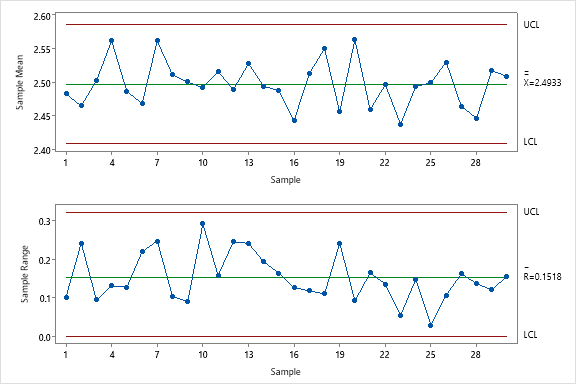
\includegraphics[width=0.5\textwidth]{Xbar_R_Paper.png}
\end{figure}


\item (14 pts) Una m\'aquina envasadora de detergente tiene 
una variabilidad natural con una desviaci\'on est\'andar de 8 ml, y la empresa 
debe garantizar que el 84.2\% de las botellas contengan al menos 500 ml para cumplir 
con la normativa de calidad. Determine a qu\'e valor promedio debe 
ajustarse la m\'aquina para que solo el 15.8\% de las botellas queden por debajo 
del contenido m\'inimo permitido.

\end{enumerate}

\newpage



\begin{center}
{An\'alisis Estad\'stico de Datos (Examen Argumentativo)}
\end{center}

Nombre: \underline{\hspace*{.2in}}
Ricardo Sánchez
\underline{\hspace*{.2in}} \quad Matr\'icula:\underline{\hspace*{.2in}}
A0000012
\underline{\hspace*{.2in}} \\

{\bf Instrucciones:} Muestra c\'omo obtienes tu respuesta. Puedes usar Excel 
o Minitab para tus cálculos de probabilidades o 
percentiles, pero no uses otros archivos o hagas uso de la IA. Respeta el 
c\'odigo de \'etica del curso y del Tecnol\'ogico 
de Monterrey.


\begin{enumerate}

\item (16 pts) Una empresa que fabrica l\'aminas de aluminio 
para la industria aeron\'autica necesita asegurar que el espesor de sus l\'aminas 
cumple con las especificaciones de $2.50 \pm 0.10$ mm. Se ha implementado una nueva 
maquinaria y se desea monitorear el espesor de las l\'aminas. Para ello, se han 
tomado muestras de tama\~no 4 cada hora y se gener\'o el diagrama que se muestra 
abajo. Calcula los l\'imites de control para el espesor de las láminas.
\begin{figure}[h!]
\centering
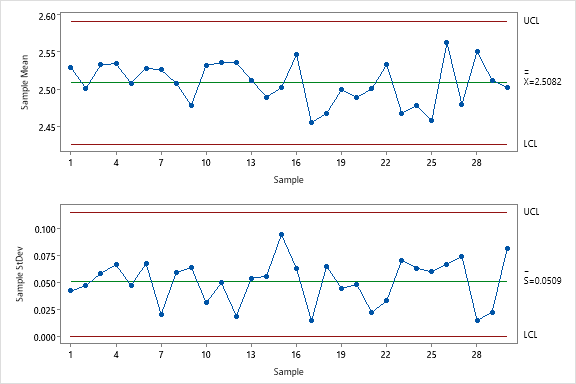
\includegraphics[width=0.5\textwidth]{Xbar_S_Paper.png}
\end{figure}


\item (14 pts) Una empresa que fabrica l\'aminas de aluminio para 
la industria aeron\'autica necesita asegurar que el espesor de sus l\'aminas cumple 
con las especificaciones de $2.50 \pm 0.10$ mm. Se ha implementado una nueva maquinaria 
y se desea monitorear el espesor de las l\'aminas. Para ello, se han tomado muestras 
de tama\~no 4 cada hora y se gener\'o el diagrama que se muestra abajo.
Calcula la probabilidad de que espesor de las láminas sea mayor 2.52 mm.
\begin{figure}[h!]
\centering
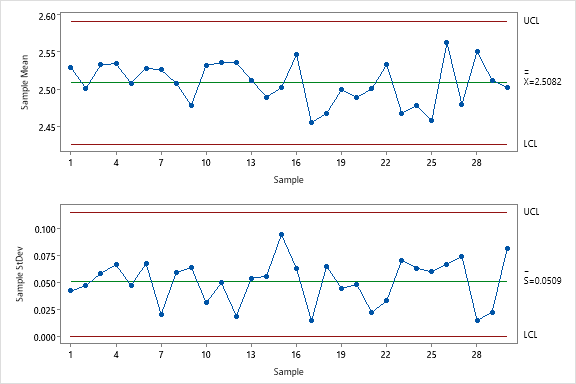
\includegraphics[width=0.5\textwidth]{Xbar_S_Paper.png}
\end{figure}


\item (14 pts) Una m\'aquina de inyecci\'on de pl\'astico 
produce piezas de precisi\'on. Se ha determinado que la probabilidad de que una 
pieza tenga una rebaba fuera de tolerancia es de $0.05$. Durante una auditor\'a 
de calidad, un inspector toma una muestra aleatoria de $n = 16$ piezas de la 
l\'inea de producci\'on. ¿Cu\'al es la probabilidad de que el inspector 
encuentre exactamente 5 piezas defectuosas en esa muestra?

\item (14 pts) En una l\'inea de producci\'on de ejes para 
motores, el di\'ametro es una caracter\'istica crítica para el ensamblaje adecuado. 
Las especificaciones del di\'ametro son $50.00 \pm 0.50$ mm. Se mide el di\'ametro 
de un eje cada 30 minutos. Despu\'es de 15 horas de mediciones, se obtuvo el 
gr\'afico IMR con un promedio m\'ovil de orden 2 que se muestra abajo.
¿Es el proceso es capaz de cumplir con las especificaciones? Argumente.
\begin{figure}[h!]
\centering
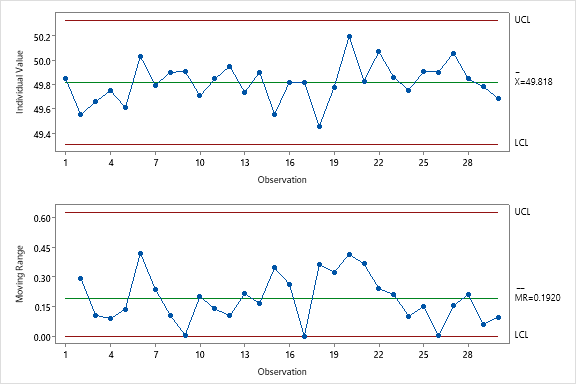
\includegraphics[width=0.5\textwidth]{IMR_Paper.png}
\end{figure}


\item (14 pts) Una empresa que fabrica tarjetas de circuitos 
impresos desea evaluar si la implementaci\'on de un nuevo sistema de ensamblaje 
ha reducido el n\'umero de disconformidades. Se tomaron 42 mediciones, antes y 
después del cambio, para analizar los efectos.
\begin{center}
\begin{tabular}{|l|c|c|}
\hline
 & Antes & Despu\'es \\ 
\hline
Media muestral & 3.60 & 2.74 \\ 
\hline
Desviaci\'on est\'andar muestral & 1.09 & 1.62 \\ 
\hline
\end{tabular}
\end{center}
¿Existe suficiente evidencia para concluir que el número medio de 
disconformidades ha disminuido despu\'es del cambio? Argumente.


\item (14 pts) Una empresa que fabrica l\'aminas de aluminio 
para la industria aeron\'autica necesita asegurar que el espesor de sus l\'aminas 
cumple con las especificaciones de $2.50 \pm 0.10$ mm. Se ha implementado una nueva 
maquinaria y se desea monitorear el espesor de las l\'aminas. Para ello, se han 
tomado muestras de tama\~no 5 cada hora y se gener\'o el diagrama que se muestra abajo.
Calcula los l\'imites de control para la {\bf variabilidad} del 
espesor de las láminas.
\begin{figure}[h!]
\centering
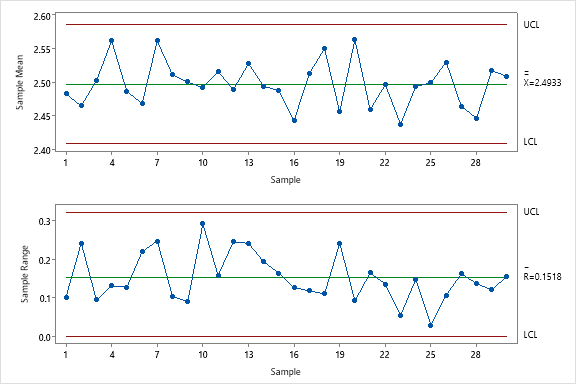
\includegraphics[width=0.5\textwidth]{Xbar_R_Paper.png}
\end{figure}


\item (14 pts) Una m\'aquina envasadora de detergente tiene 
una variabilidad natural con una desviaci\'on est\'andar de 8 ml, y la empresa 
debe garantizar que el 91.9\% de las botellas contengan al menos 500 ml para cumplir 
con la normativa de calidad. Determine a qu\'e valor promedio debe 
ajustarse la m\'aquina para que solo el 8.1\% de las botellas queden por debajo 
del contenido m\'inimo permitido.

\end{enumerate}

\newpage



\begin{center}
{An\'alisis Estad\'stico de Datos (Examen Argumentativo)}
\end{center}

Nombre: \underline{\hspace*{.2in}}
Paola Navarro
\underline{\hspace*{.2in}} \quad Matr\'icula:\underline{\hspace*{.2in}}
A0000013
\underline{\hspace*{.2in}} \\

{\bf Instrucciones:} Muestra c\'omo obtienes tu respuesta. Puedes usar Excel 
o Minitab para tus cálculos de probabilidades o 
percentiles, pero no uses otros archivos o hagas uso de la IA. Respeta el 
c\'odigo de \'etica del curso y del Tecnol\'ogico 
de Monterrey.


\begin{enumerate}

\item (16 pts) Una empresa que fabrica l\'aminas de aluminio 
para la industria aeron\'autica necesita asegurar que el espesor de sus l\'aminas 
cumple con las especificaciones de $2.50 \pm 0.10$ mm. Se ha implementado una nueva 
maquinaria y se desea monitorear el espesor de las l\'aminas. Para ello, se han 
tomado muestras de tama\~no 4 cada hora y se gener\'o el diagrama que se muestra 
abajo. Calcula los l\'imites de control para el espesor de las láminas.
\begin{figure}[h!]
\centering
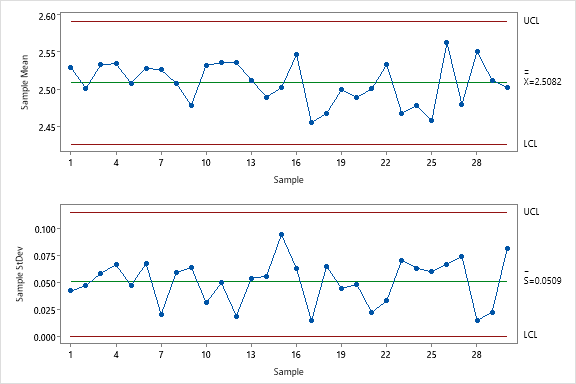
\includegraphics[width=0.5\textwidth]{Xbar_S_Paper.png}
\end{figure}


\item (14 pts) En una l\'inea de producci\'on de ejes para 
motores, el di\'ametro es una caracter\'istica crítica para el ensamblaje adecuado. 
Las especificaciones del di\'ametro son $50.00 \pm 0.50$ mm. Se mide el di\'ametro 
de un eje cada 30 minutos. Despu\'es de 15 horas de mediciones, se obtuvo el 
gr\'afico IMR con un promedio m\'ovil de orden 2 que se muestra abajo.
Calcula la probabilidad de que di\'ametro del eje se encuentre entre 49.9 mm y 
50.0 mm.
\begin{figure}[h!]
\centering
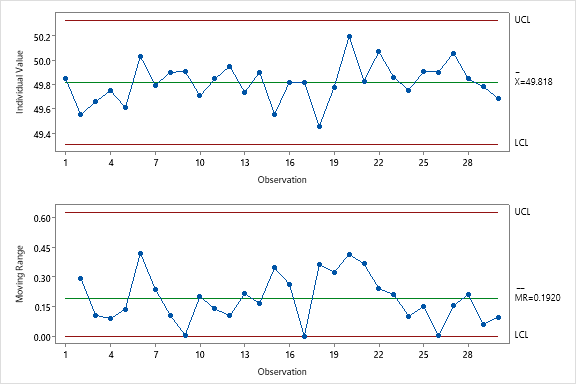
\includegraphics[width=0.5\textwidth]{IMR_Paper.png}
\end{figure}


\item (14 pts) Una m\'aquina de inyecci\'on de pl\'astico 
produce piezas de precisi\'on. Se ha determinado que la probabilidad de que una 
pieza tenga una rebaba fuera de tolerancia es de $0.05$. Durante una auditor\'a 
de calidad, un inspector toma una muestra aleatoria de $n = 13$ piezas de la 
l\'inea de producci\'on. ¿Cu\'al es la probabilidad de que el inspector 
encuentre exactamente 6 piezas defectuosas en esa muestra?

\item (14 pts) En una l\'inea de producci\'on de ejes para 
motores, el di\'ametro es una caracter\'istica crítica para el ensamblaje adecuado. 
Las especificaciones del di\'ametro son $50.00 \pm 0.50$ mm. Se mide el di\'ametro 
de un eje cada 30 minutos. Despu\'es de 15 horas de mediciones, se obtuvo el 
gr\'afico IMR con un promedio m\'ovil de orden 2 que se muestra abajo.
¿Es el proceso es capaz de cumplir con las especificaciones? Argumente.
\begin{figure}[h!]
\centering
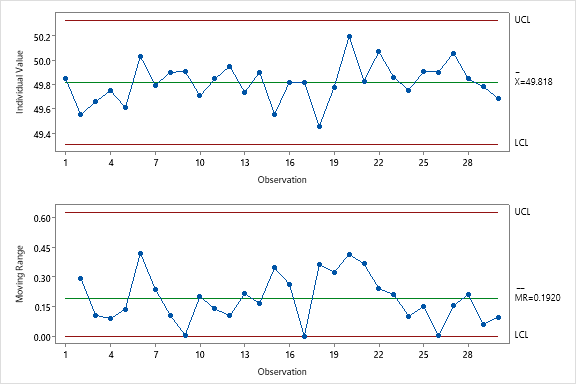
\includegraphics[width=0.5\textwidth]{IMR_Paper.png}
\end{figure}


\item (14 pts) Una empresa que fabrica tarjetas de circuitos 
impresos desea evaluar si la implementaci\'on de un nuevo sistema de ensamblaje 
ha reducido el n\'umero de disconformidades. Se tomaron 42 mediciones, antes y 
después del cambio, para analizar los efectos.
\begin{center}
\begin{tabular}{|l|c|c|}
\hline
 & Antes & Despu\'es \\ 
\hline
Media muestral & 3.60 & 3.44 \\ 
\hline
Desviaci\'on est\'andar muestral & 1.09 & 1.62 \\ 
\hline
\end{tabular}
\end{center}
¿Existe suficiente evidencia para concluir que el número medio de 
disconformidades ha disminuido despu\'es del cambio? Argumente.


\item (14 pts) Una empresa que fabrica l\'aminas de aluminio 
para la industria aeron\'autica necesita asegurar que el espesor de sus l\'aminas 
cumple con las especificaciones de $2.50 \pm 0.10$ mm. Se ha implementado una nueva 
maquinaria y se desea monitorear el espesor de las l\'aminas. Para ello, se han 
tomado muestras de tama\~no 5 cada hora y se gener\'o el diagrama que se muestra abajo.
Calcula los l\'imites de control para la {\bf variabilidad} del 
espesor de las láminas.
\begin{figure}[h!]
\centering
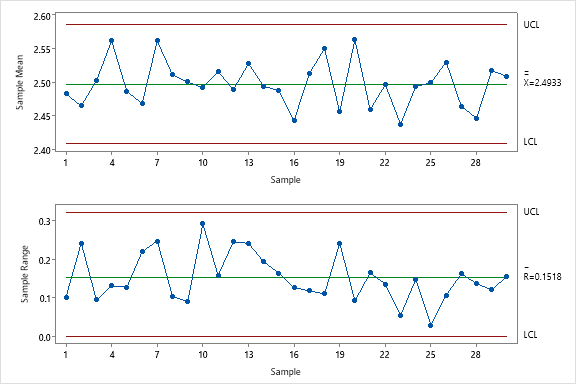
\includegraphics[width=0.5\textwidth]{Xbar_R_Paper.png}
\end{figure}


\item (14 pts) Una m\'aquina envasadora de detergente tiene 
una variabilidad natural con una desviaci\'on est\'andar de 8 ml, y la empresa 
debe garantizar que el 95.8\% de las botellas contengan al menos 500 ml para cumplir 
con la normativa de calidad. Determine a qu\'e valor promedio debe 
ajustarse la m\'aquina para que solo el 4.2\% de las botellas queden por debajo 
del contenido m\'inimo permitido.

\end{enumerate}

\newpage



\begin{center}
{An\'alisis Estad\'stico de Datos (Examen Argumentativo)}
\end{center}

Nombre: \underline{\hspace*{.2in}}
Javier Ramírez
\underline{\hspace*{.2in}} \quad Matr\'icula:\underline{\hspace*{.2in}}
A0000014
\underline{\hspace*{.2in}} \\

{\bf Instrucciones:} Muestra c\'omo obtienes tu respuesta. Puedes usar Excel 
o Minitab para tus cálculos de probabilidades o 
percentiles, pero no uses otros archivos o hagas uso de la IA. Respeta el 
c\'odigo de \'etica del curso y del Tecnol\'ogico 
de Monterrey.


\begin{enumerate}

\item (16 pts) En una l\'inea de producci\'on de ejes para 
motores, el di\'ametro es una caracter\'istica crítica para el ensamblaje adecuado. 
Las especificaciones del di\'ametro son $50.00 \pm 0.50$ mm. Se mide el di\'ametro 
de un eje cada 30 minutos. Despu\'es de 15 horas de mediciones, se obtuvo el 
gr\'afico IMR con un promedio m\'ovil de orden 2 que se muestra abajo. 
Calcula los l\'imites de control para el di\'ametro del eje.
\begin{figure}[h!]
\centering
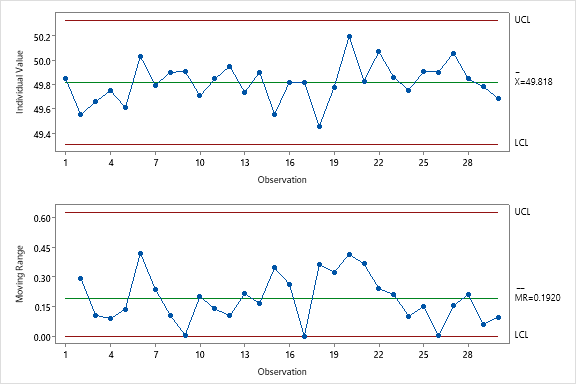
\includegraphics[width=0.5\textwidth]{IMR_Paper.png}
\end{figure}


\item (14 pts) En una l\'inea de producci\'on de ejes para 
motores, el di\'ametro es una caracter\'istica crítica para el ensamblaje adecuado. 
Las especificaciones del di\'ametro son $50.00 \pm 0.50$ mm. Se mide el di\'ametro 
de un eje cada 30 minutos. Despu\'es de 15 horas de mediciones, se obtuvo el 
gr\'afico IMR con un promedio m\'ovil de orden 2 que se muestra abajo.
Calcula la probabilidad de que di\'ametro del eje se encuentre entre 49.6 mm y 
50.3 mm.
\begin{figure}[h!]
\centering
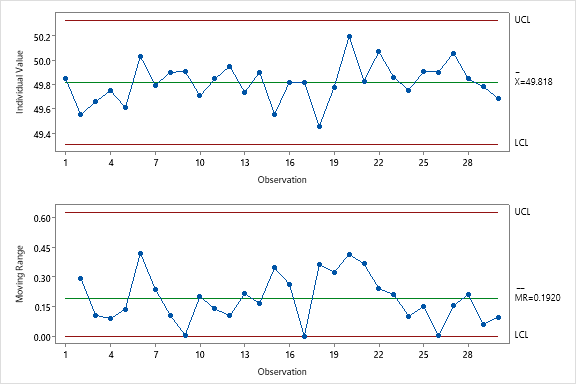
\includegraphics[width=0.5\textwidth]{IMR_Paper.png}
\end{figure}


\item (14 pts) Una m\'aquina de inyecci\'on de pl\'astico 
produce piezas de precisi\'on. Se ha determinado que la probabilidad de que una 
pieza tenga una rebaba fuera de tolerancia es de $0.05$. Durante una auditor\'a 
de calidad, un inspector toma una muestra aleatoria de $n = 13$ piezas de la 
l\'inea de producci\'on. ¿Cu\'al es la probabilidad de que el inspector 
encuentre exactamente 4 piezas defectuosas en esa muestra?

\item (14 pts) En una l\'inea de producci\'on de ejes para 
motores, el di\'ametro es una caracter\'istica crítica para el ensamblaje adecuado. 
Las especificaciones del di\'ametro son $50.00 \pm 0.50$ mm. Se mide el di\'ametro 
de un eje cada 30 minutos. Despu\'es de 15 horas de mediciones, se obtuvo el 
gr\'afico IMR con un promedio m\'ovil de orden 2 que se muestra abajo.
¿Es el proceso es capaz de cumplir con las especificaciones? Argumente.
\begin{figure}[h!]
\centering
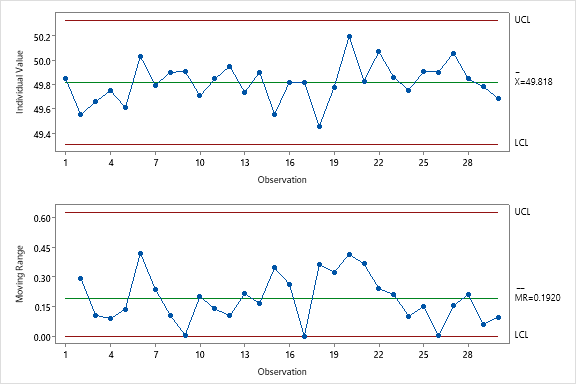
\includegraphics[width=0.5\textwidth]{IMR_Paper.png}
\end{figure}


\item (14 pts) Una empresa que fabrica tarjetas de circuitos 
impresos desea evaluar si la implementaci\'on de un nuevo sistema de ensamblaje 
ha reducido el n\'umero de disconformidades. Se tomaron 50 mediciones, antes y 
después del cambio, para analizar los efectos.
\begin{center}
\begin{tabular}{|l|c|c|}
\hline
 & Antes & Despu\'es \\ 
\hline
Media muestral & 3.60 & 3.02 \\ 
\hline
Desviaci\'on est\'andar muestral & 1.09 & 1.62 \\ 
\hline
\end{tabular}
\end{center}
Calcula un intervalo de confianza de 98\% para el número medio 
de disconformidades antes del cambio. Interprete su resultado.


\item (14 pts) Una empresa que fabrica l\'aminas de aluminio 
para la industria aeron\'autica necesita asegurar que el espesor de sus l\'aminas 
cumple con las especificaciones de $2.50 \pm 0.10$ mm. Se ha implementado una nueva 
maquinaria y se desea monitorear el espesor de las l\'aminas. Para ello, se han 
tomado muestras de tama\~no 5 cada hora y se gener\'o el diagrama que se muestra abajo.
Calcula los l\'imites de control para la {\bf variabilidad} del 
espesor de las láminas.
\begin{figure}[h!]
\centering
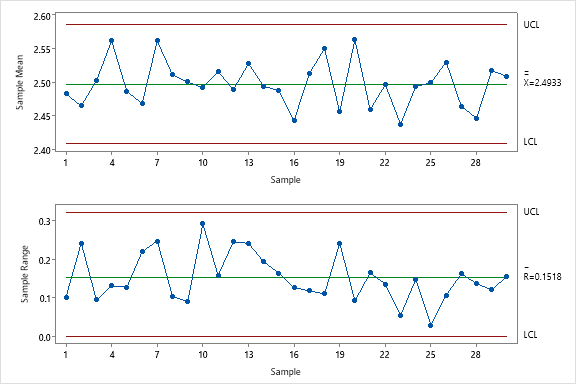
\includegraphics[width=0.5\textwidth]{Xbar_R_Paper.png}
\end{figure}


\item (14 pts) Una m\'aquina envasadora de detergente tiene 
una variabilidad natural con una desviaci\'on est\'andar de 8 ml, y la empresa 
debe garantizar que el 82.1\% de las botellas contengan al menos 500 ml para cumplir 
con la normativa de calidad. Determine a qu\'e valor promedio debe 
ajustarse la m\'aquina para que solo el 17.9\% de las botellas queden por debajo 
del contenido m\'inimo permitido.

\end{enumerate}

\newpage



\begin{center}
{An\'alisis Estad\'stico de Datos (Examen Argumentativo)}
\end{center}

Nombre: \underline{\hspace*{.2in}}
Karla Jiménez
\underline{\hspace*{.2in}} \quad Matr\'icula:\underline{\hspace*{.2in}}
A0000015
\underline{\hspace*{.2in}} \\

{\bf Instrucciones:} Muestra c\'omo obtienes tu respuesta. Puedes usar Excel 
o Minitab para tus cálculos de probabilidades o 
percentiles, pero no uses otros archivos o hagas uso de la IA. Respeta el 
c\'odigo de \'etica del curso y del Tecnol\'ogico 
de Monterrey.


\begin{enumerate}

\item (16 pts) Una empresa que fabrica l\'aminas de aluminio 
para la industria aeron\'autica necesita asegurar que el espesor de sus l\'aminas 
cumple con las especificaciones de $2.50 \pm 0.10$ mm. Se ha implementado una nueva 
maquinaria y se desea monitorear el espesor de las l\'aminas. Para ello, se han 
tomado muestras de tama\~no 4 cada hora y se gener\'o el diagrama que se muestra 
abajo. Calcula los l\'imites de control para el espesor de las láminas.
\begin{figure}[h!]
\centering
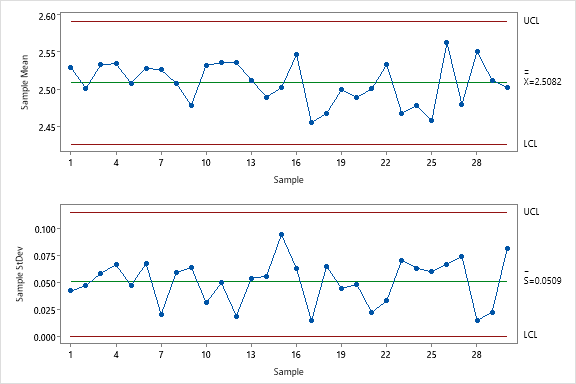
\includegraphics[width=0.5\textwidth]{Xbar_S_Paper.png}
\end{figure}


\item (14 pts) Una empresa que fabrica l\'aminas de aluminio para 
la industria aeron\'autica necesita asegurar que el espesor de sus l\'aminas cumple 
con las especificaciones de $2.50 \pm 0.10$ mm. Se ha implementado una nueva maquinaria 
y se desea monitorear el espesor de las l\'aminas. Para ello, se han tomado muestras 
de tama\~no 4 cada hora y se gener\'o el diagrama que se muestra abajo.
Calcula la probabilidad de que espesor de las láminas sea mayor 2.54 mm.
\begin{figure}[h!]
\centering
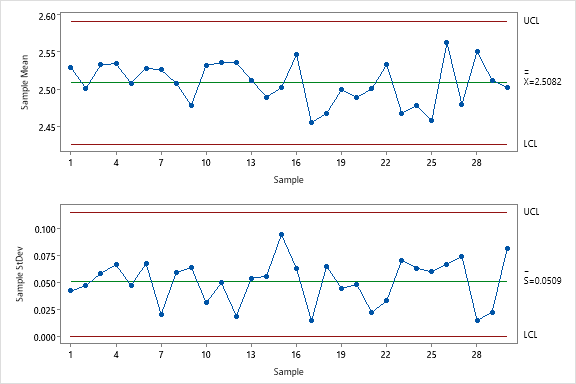
\includegraphics[width=0.5\textwidth]{Xbar_S_Paper.png}
\end{figure}


\item (14 pts) Una m\'aquina de inyecci\'on de pl\'astico 
produce piezas de precisi\'on. Se ha determinado que la probabilidad de que una 
pieza tenga una rebaba fuera de tolerancia es de $0.05$. Durante una auditor\'a 
de calidad, un inspector toma una muestra aleatoria de $n = 16$ piezas de la 
l\'inea de producci\'on. ¿Cu\'al es la probabilidad de que el inspector 
encuentre exactamente 7 piezas defectuosas en esa muestra?

\item (14 pts) En una l\'inea de producci\'on de ejes para 
motores, el di\'ametro es una caracter\'istica crítica para el ensamblaje adecuado. 
Las especificaciones del di\'ametro son $50.00 \pm 0.60$ mm. Se mide el di\'ametro 
de un eje cada 30 minutos. Despu\'es de 15 horas de mediciones, se obtuvo el 
gr\'afico IMR con un promedio m\'ovil de orden 2 que se muestra abajo.
¿Es el proceso es capaz de cumplir con las especificaciones? Argumente.
\begin{figure}[h!]
\centering
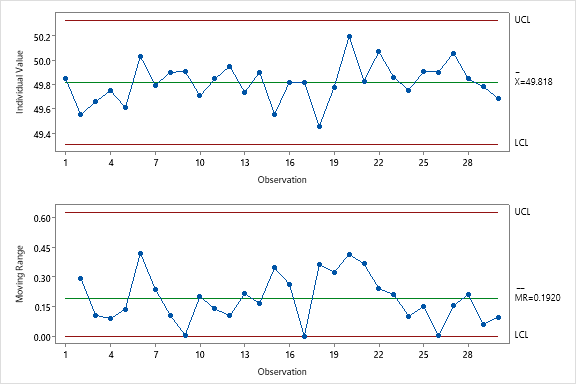
\includegraphics[width=0.5\textwidth]{IMR_Paper.png}
\end{figure}


\item (14 pts) Una empresa que fabrica tarjetas de circuitos 
impresos desea evaluar si la implementaci\'on de un nuevo sistema de ensamblaje 
ha reducido el n\'umero de disconformidades. Se tomaron 46 mediciones, antes y 
después del cambio, para analizar los efectos.
\begin{center}
\begin{tabular}{|l|c|c|}
\hline
 & Antes & Despu\'es \\ 
\hline
Media muestral & 3.60 & 3.29 \\ 
\hline
Desviaci\'on est\'andar muestral & 1.09 & 1.62 \\ 
\hline
\end{tabular}
\end{center}
Calcula un intervalo de confianza de 93\% para el número medio 
de disconformidades antes del cambio. Interprete su resultado.


\item (14 pts) Una empresa que fabrica l\'aminas de aluminio para 
la industria aeron\'autica necesita asegurar que el espesor de sus l\'aminas cumple 
con las especificaciones de $2.50 \pm 0.10$ mm. Se ha implementado una nueva maquinaria 
y se desea monitorear el espesor de las l\'aminas. Para ello, se han tomado muestras 
de tama\~no 4 cada hora y se gener\'o el diagrama que se muestra abajo.
Calcula los l\'imites de control para la {\bf variabilidad} del 
espesor de las láminas.
\begin{figure}[h!]
\centering
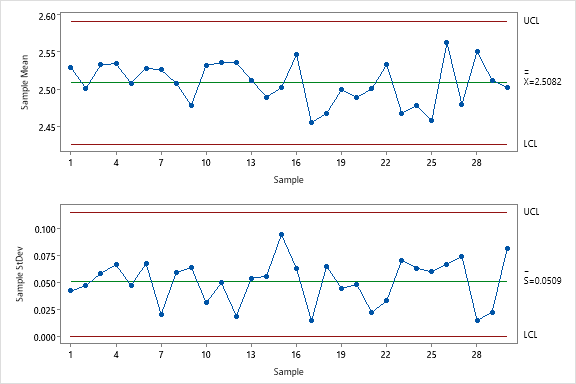
\includegraphics[width=0.5\textwidth]{Xbar_S_Paper.png}
\end{figure}


\item (14 pts) Una m\'aquina envasadora de detergente tiene 
una variabilidad natural con una desviaci\'on est\'andar de 8 ml, y la empresa 
debe garantizar que el 86.1\% de las botellas contengan al menos 500 ml para cumplir 
con la normativa de calidad. Determine a qu\'e valor promedio debe 
ajustarse la m\'aquina para que solo el 13.9\% de las botellas queden por debajo 
del contenido m\'inimo permitido.

\end{enumerate}

\newpage



\begin{center}
{An\'alisis Estad\'stico de Datos (Examen Argumentativo)}
\end{center}

Nombre: \underline{\hspace*{.2in}}
Sebastián Flores
\underline{\hspace*{.2in}} \quad Matr\'icula:\underline{\hspace*{.2in}}
A0000016
\underline{\hspace*{.2in}} \\

{\bf Instrucciones:} Muestra c\'omo obtienes tu respuesta. Puedes usar Excel 
o Minitab para tus cálculos de probabilidades o 
percentiles, pero no uses otros archivos o hagas uso de la IA. Respeta el 
c\'odigo de \'etica del curso y del Tecnol\'ogico 
de Monterrey.


\begin{enumerate}

\item (16 pts) Una empresa que fabrica l\'aminas de aluminio 
para la industria aeron\'autica necesita asegurar que el espesor de sus l\'aminas 
cumple con las especificaciones de $2.50 \pm 0.10$ mm. Se ha implementado una nueva 
maquinaria y se desea monitorear el espesor de las l\'aminas. Para ello, se han 
tomado muestras de tama\~no 4 cada hora y se gener\'o el diagrama que se muestra 
abajo. Calcula los l\'imites de control para el espesor de las láminas.
\begin{figure}[h!]
\centering
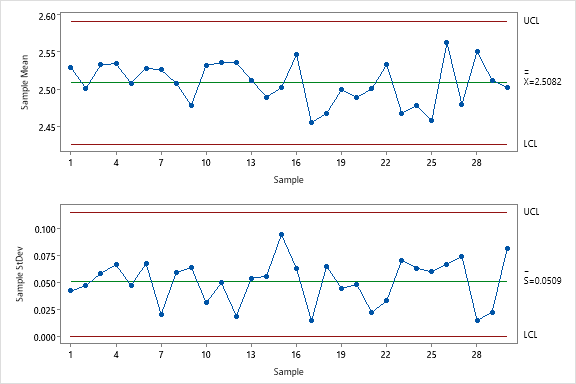
\includegraphics[width=0.5\textwidth]{Xbar_S_Paper.png}
\end{figure}


\item (14 pts) En una l\'inea de producci\'on de ejes para 
motores, el di\'ametro es una caracter\'istica crítica para el ensamblaje adecuado. 
Las especificaciones del di\'ametro son $50.00 \pm 0.50$ mm. Se mide el di\'ametro 
de un eje cada 30 minutos. Despu\'es de 15 horas de mediciones, se obtuvo el 
gr\'afico IMR con un promedio m\'ovil de orden 2 que se muestra abajo.
Calcula la probabilidad de que di\'ametro del eje se encuentre entre 49.8 mm y 
50.4 mm.
\begin{figure}[h!]
\centering
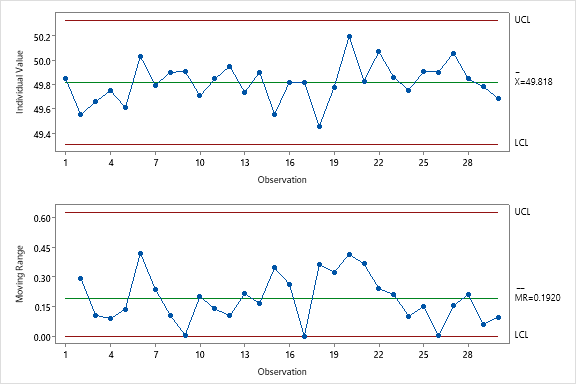
\includegraphics[width=0.5\textwidth]{IMR_Paper.png}
\end{figure}


\item (14 pts) Una m\'aquina de inyecci\'on de pl\'astico 
produce piezas de precisi\'on. Se ha determinado que la probabilidad de que una 
pieza tenga una rebaba fuera de tolerancia es de $0.05$. Durante una auditor\'a 
de calidad, un inspector toma una muestra aleatoria de $n = 15$ piezas de la 
l\'inea de producci\'on. ¿Cu\'al es la probabilidad de que el inspector 
encuentre exactamente 6 piezas defectuosas en esa muestra?

\item (14 pts) Una empresa que fabrica l\'aminas de aluminio para 
la industria aeron\'autica necesita asegurar que el espesor de sus l\'aminas cumple 
con las especificaciones de $2.50 \pm 0.10$ mm. Se ha implementado una nueva maquinaria 
y se desea monitorear el espesor de las l\'aminas. Para ello, se han tomado muestras 
de tama\~no 4 cada hora y se gener\'o el diagrama que se muestra abajo.
¿Es el proceso es capaz de cumplir con las especificaciones? Argumente.
\begin{figure}[h!]
\centering
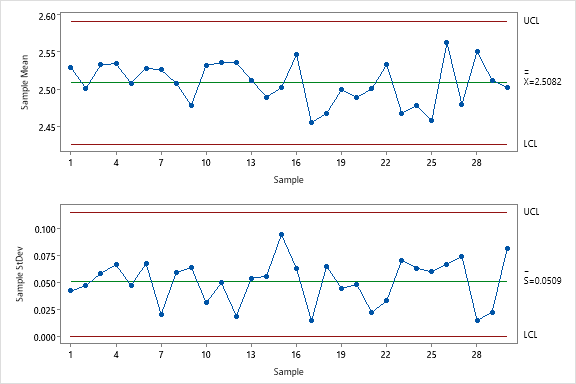
\includegraphics[width=0.5\textwidth]{Xbar_S_Paper.png}
\end{figure}


\item (14 pts) Una empresa que fabrica tarjetas de circuitos 
impresos desea evaluar si la implementaci\'on de un nuevo sistema de ensamblaje 
ha reducido el n\'umero de disconformidades. Se tomaron 38 mediciones, antes y 
después del cambio, para analizar los efectos.
\begin{center}
\begin{tabular}{|l|c|c|}
\hline
 & Antes & Despu\'es \\ 
\hline
Media muestral & 3.60 & 2.74 \\ 
\hline
Desviaci\'on est\'andar muestral & 1.09 & 1.62 \\ 
\hline
\end{tabular}
\end{center}
¿Existe suficiente evidencia para concluir que el número medio de 
disconformidades ha disminuido despu\'es del cambio? Argumente.


\item (14 pts) Una empresa que fabrica l\'aminas de aluminio para 
la industria aeron\'autica necesita asegurar que el espesor de sus l\'aminas cumple 
con las especificaciones de $2.50 \pm 0.10$ mm. Se ha implementado una nueva maquinaria 
y se desea monitorear el espesor de las l\'aminas. Para ello, se han tomado muestras 
de tama\~no 4 cada hora y se gener\'o el diagrama que se muestra abajo.
Calcula los l\'imites de control para la {\bf variabilidad} del 
espesor de las láminas.
\begin{figure}[h!]
\centering
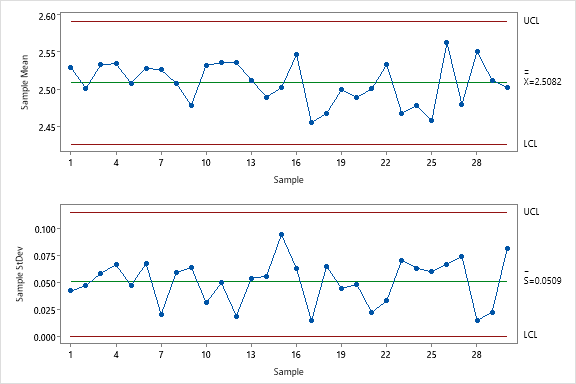
\includegraphics[width=0.5\textwidth]{Xbar_S_Paper.png}
\end{figure}


\item (14 pts) Una m\'aquina envasadora de detergente tiene 
una variabilidad natural con una desviaci\'on est\'andar de 8 ml, y la empresa 
debe garantizar que el 92.0\% de las botellas contengan al menos 500 ml para cumplir 
con la normativa de calidad. Determine a qu\'e valor promedio debe 
ajustarse la m\'aquina para que solo el 8.0\% de las botellas queden por debajo 
del contenido m\'inimo permitido.

\end{enumerate}

\newpage



\begin{center}
{An\'alisis Estad\'stico de Datos (Examen Argumentativo)}
\end{center}

Nombre: \underline{\hspace*{.2in}}
Natalia Moreno
\underline{\hspace*{.2in}} \quad Matr\'icula:\underline{\hspace*{.2in}}
A0000017
\underline{\hspace*{.2in}} \\

{\bf Instrucciones:} Muestra c\'omo obtienes tu respuesta. Puedes usar Excel 
o Minitab para tus cálculos de probabilidades o 
percentiles, pero no uses otros archivos o hagas uso de la IA. Respeta el 
c\'odigo de \'etica del curso y del Tecnol\'ogico 
de Monterrey.


\begin{enumerate}

\item (16 pts) En una l\'inea de producci\'on de ejes para 
motores, el di\'ametro es una caracter\'istica crítica para el ensamblaje adecuado. 
Las especificaciones del di\'ametro son $50.00 \pm 0.50$ mm. Se mide el di\'ametro 
de un eje cada 30 minutos. Despu\'es de 15 horas de mediciones, se obtuvo el 
gr\'afico IMR con un promedio m\'ovil de orden 2 que se muestra abajo. 
Calcula los l\'imites de control para el di\'ametro del eje.
\begin{figure}[h!]
\centering
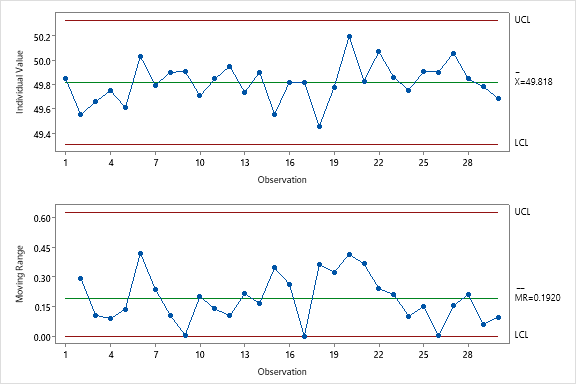
\includegraphics[width=0.5\textwidth]{IMR_Paper.png}
\end{figure}


\item (14 pts) En una l\'inea de producci\'on de ejes para 
motores, el di\'ametro es una caracter\'istica crítica para el ensamblaje adecuado. 
Las especificaciones del di\'ametro son $50.00 \pm 0.50$ mm. Se mide el di\'ametro 
de un eje cada 30 minutos. Despu\'es de 15 horas de mediciones, se obtuvo el 
gr\'afico IMR con un promedio m\'ovil de orden 2 que se muestra abajo.
Calcula la probabilidad de que di\'ametro del eje se encuentre entre 49.7 mm y 
50.0 mm.
\begin{figure}[h!]
\centering
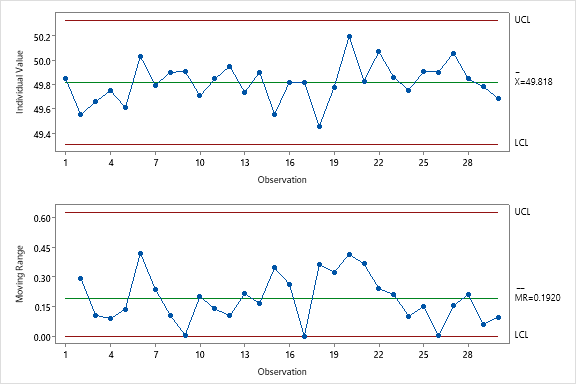
\includegraphics[width=0.5\textwidth]{IMR_Paper.png}
\end{figure}


\item (14 pts) Una m\'aquina de inyecci\'on de pl\'astico 
produce piezas de precisi\'on. Se ha determinado que la probabilidad de que una 
pieza tenga una rebaba fuera de tolerancia es de $0.05$. Durante una auditor\'a 
de calidad, un inspector toma una muestra aleatoria de $n = 15$ piezas de la 
l\'inea de producci\'on. ¿Cu\'al es la probabilidad de que el inspector 
encuentre exactamente 6 piezas defectuosas en esa muestra?

\item (14 pts) Una empresa que fabrica l\'aminas de aluminio para 
la industria aeron\'autica necesita asegurar que el espesor de sus l\'aminas cumple 
con las especificaciones de $2.50 \pm 0.10$ mm. Se ha implementado una nueva maquinaria 
y se desea monitorear el espesor de las l\'aminas. Para ello, se han tomado muestras 
de tama\~no 4 cada hora y se gener\'o el diagrama que se muestra abajo.
¿Es el proceso es capaz de cumplir con las especificaciones? Argumente.
\begin{figure}[h!]
\centering
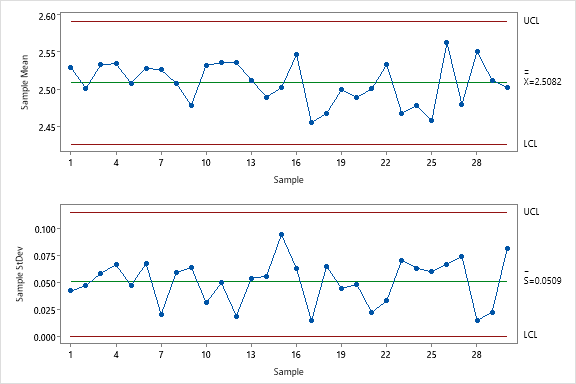
\includegraphics[width=0.5\textwidth]{Xbar_S_Paper.png}
\end{figure}


\item (14 pts) Una empresa que fabrica tarjetas de circuitos 
impresos desea evaluar si la implementaci\'on de un nuevo sistema de ensamblaje 
ha reducido el n\'umero de disconformidades. Se tomaron 38 mediciones, antes y 
después del cambio, para analizar los efectos.
\begin{center}
\begin{tabular}{|l|c|c|}
\hline
 & Antes & Despu\'es \\ 
\hline
Media muestral & 3.60 & 3.53 \\ 
\hline
Desviaci\'on est\'andar muestral & 1.09 & 1.62 \\ 
\hline
\end{tabular}
\end{center}
Calcula un intervalo de confianza de 97\% para el número medio 
de disconformidades antes del cambio. Interprete su resultado.


\item (14 pts) Una empresa que fabrica l\'aminas de aluminio 
para la industria aeron\'autica necesita asegurar que el espesor de sus l\'aminas 
cumple con las especificaciones de $2.50 \pm 0.10$ mm. Se ha implementado una nueva 
maquinaria y se desea monitorear el espesor de las l\'aminas. Para ello, se han 
tomado muestras de tama\~no 5 cada hora y se gener\'o el diagrama que se muestra abajo.
Calcula los l\'imites de control para la {\bf variabilidad} del 
espesor de las láminas.
\begin{figure}[h!]
\centering
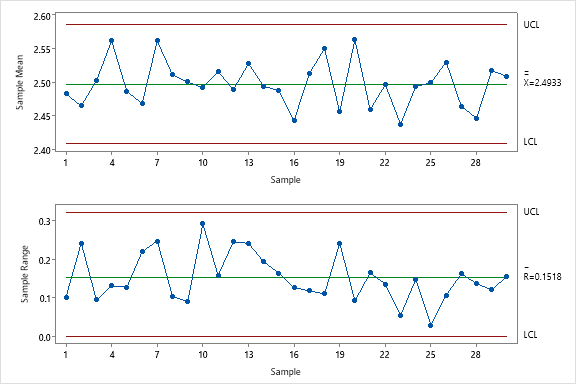
\includegraphics[width=0.5\textwidth]{Xbar_R_Paper.png}
\end{figure}


\item (14 pts) Una m\'aquina envasadora de detergente tiene 
una variabilidad natural con una desviaci\'on est\'andar de 8 ml, y la empresa 
debe garantizar que el 89.8\% de las botellas contengan al menos 500 ml para cumplir 
con la normativa de calidad. Determine a qu\'e valor promedio debe 
ajustarse la m\'aquina para que solo el 10.2\% de las botellas queden por debajo 
del contenido m\'inimo permitido.

\end{enumerate}

\newpage



\begin{center}
{An\'alisis Estad\'stico de Datos (Examen Argumentativo)}
\end{center}

Nombre: \underline{\hspace*{.2in}}
Alejandro Ortiz
\underline{\hspace*{.2in}} \quad Matr\'icula:\underline{\hspace*{.2in}}
A0000018
\underline{\hspace*{.2in}} \\

{\bf Instrucciones:} Muestra c\'omo obtienes tu respuesta. Puedes usar Excel 
o Minitab para tus cálculos de probabilidades o 
percentiles, pero no uses otros archivos o hagas uso de la IA. Respeta el 
c\'odigo de \'etica del curso y del Tecnol\'ogico 
de Monterrey.


\begin{enumerate}

\item (16 pts) Una empresa que fabrica l\'aminas de aluminio 
para la industria aeron\'autica necesita asegurar que el espesor de sus l\'aminas 
cumple con las especificaciones de $2.50 \pm 0.10$ mm. Se ha implementado una nueva 
maquinaria y se desea monitorear el espesor de las l\'aminas. Para ello, se han tomado 
muestras de tama\~no 5 cada hora y se gener\'o el diagrama que se muestra abajo.
Calcula los l\'imites de control para el espesor de las láminas.
\begin{figure}[h!]
\centering
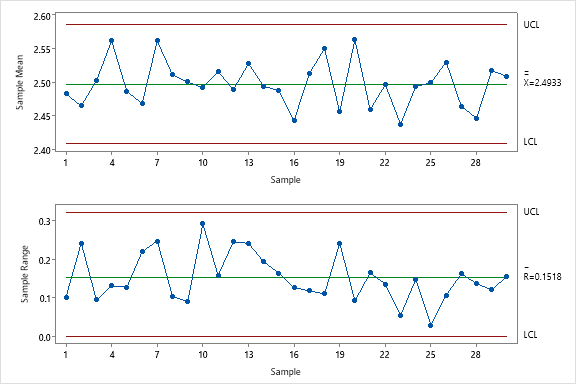
\includegraphics[width=0.5\textwidth]{Xbar_R_Paper.png}
\end{figure}


\item (14 pts) En una l\'inea de producci\'on de ejes para 
motores, el di\'ametro es una caracter\'istica crítica para el ensamblaje adecuado. 
Las especificaciones del di\'ametro son $50.00 \pm 0.50$ mm. Se mide el di\'ametro 
de un eje cada 30 minutos. Despu\'es de 15 horas de mediciones, se obtuvo el 
gr\'afico IMR con un promedio m\'ovil de orden 2 que se muestra abajo.
Calcula la probabilidad de que di\'ametro del eje se encuentre entre 49.9 mm y 
50.2 mm.
\begin{figure}[h!]
\centering
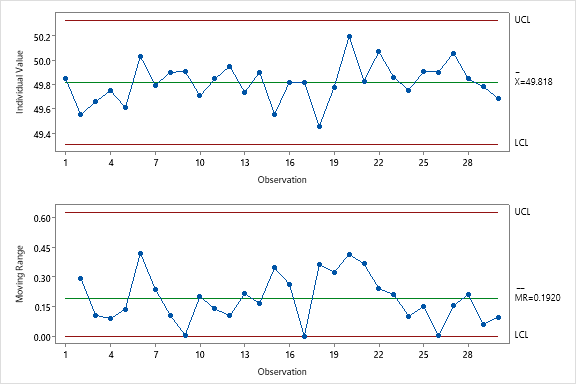
\includegraphics[width=0.5\textwidth]{IMR_Paper.png}
\end{figure}


\item (14 pts) Una m\'aquina de inyecci\'on de pl\'astico 
produce piezas de precisi\'on. Se ha determinado que la probabilidad de que una 
pieza tenga una rebaba fuera de tolerancia es de $0.05$. Durante una auditor\'a 
de calidad, un inspector toma una muestra aleatoria de $n = 16$ piezas de la 
l\'inea de producci\'on. ¿Cu\'al es la probabilidad de que el inspector 
encuentre exactamente 4 piezas defectuosas en esa muestra?

\item (14 pts) Una empresa que fabrica l\'aminas de aluminio para 
la industria aeron\'autica necesita asegurar que el espesor de sus l\'aminas cumple 
con las especificaciones de $2.50 \pm 0.10$ mm. Se ha implementado una nueva maquinaria 
y se desea monitorear el espesor de las l\'aminas. Para ello, se han tomado muestras 
de tama\~no 4 cada hora y se gener\'o el diagrama que se muestra abajo.
¿Es el proceso es capaz de cumplir con las especificaciones? Argumente.
\begin{figure}[h!]
\centering
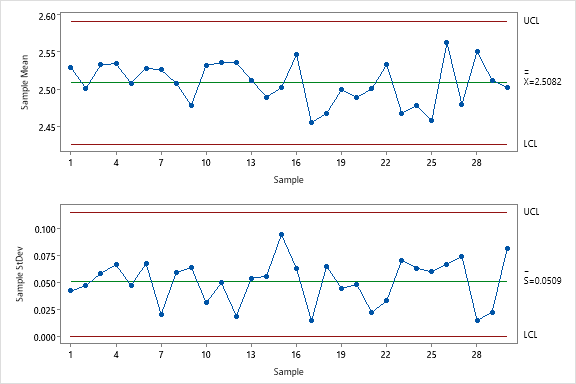
\includegraphics[width=0.5\textwidth]{Xbar_S_Paper.png}
\end{figure}


\item (14 pts) Una empresa que fabrica tarjetas de circuitos 
impresos desea evaluar si la implementaci\'on de un nuevo sistema de ensamblaje 
ha reducido el n\'umero de disconformidades. Se tomaron 36 mediciones, antes y 
después del cambio, para analizar los efectos.
\begin{center}
\begin{tabular}{|l|c|c|}
\hline
 & Antes & Despu\'es \\ 
\hline
Media muestral & 3.60 & 3.28 \\ 
\hline
Desviaci\'on est\'andar muestral & 1.09 & 1.62 \\ 
\hline
\end{tabular}
\end{center}
Calcula un intervalo de confianza de 92\% para el número medio 
de disconformidades antes del cambio. Interprete su resultado.


\item (14 pts) Una empresa que fabrica l\'aminas de aluminio para 
la industria aeron\'autica necesita asegurar que el espesor de sus l\'aminas cumple 
con las especificaciones de $2.50 \pm 0.10$ mm. Se ha implementado una nueva maquinaria 
y se desea monitorear el espesor de las l\'aminas. Para ello, se han tomado muestras 
de tama\~no 4 cada hora y se gener\'o el diagrama que se muestra abajo.
Calcula los l\'imites de control para la {\bf variabilidad} del 
espesor de las láminas.
\begin{figure}[h!]
\centering
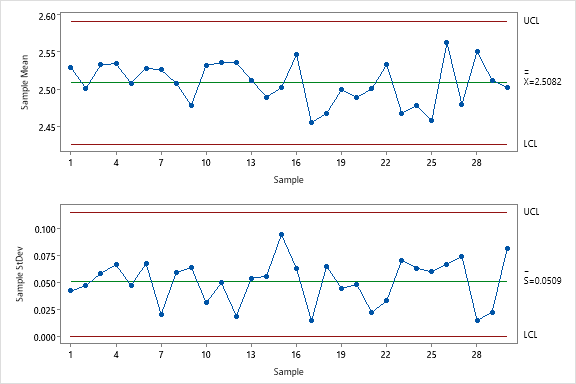
\includegraphics[width=0.5\textwidth]{Xbar_S_Paper.png}
\end{figure}


\item (14 pts) Una m\'aquina envasadora de detergente tiene 
una variabilidad natural con una desviaci\'on est\'andar de 8 ml, y la empresa 
debe garantizar que el 84.1\% de las botellas contengan al menos 500 ml para cumplir 
con la normativa de calidad. Determine a qu\'e valor promedio debe 
ajustarse la m\'aquina para que solo el 15.9\% de las botellas queden por debajo 
del contenido m\'inimo permitido.

\end{enumerate}

\newpage



\begin{center}
{An\'alisis Estad\'stico de Datos (Examen Argumentativo)}
\end{center}

Nombre: \underline{\hspace*{.2in}}
Camila Salazar
\underline{\hspace*{.2in}} \quad Matr\'icula:\underline{\hspace*{.2in}}
A0000019
\underline{\hspace*{.2in}} \\

{\bf Instrucciones:} Muestra c\'omo obtienes tu respuesta. Puedes usar Excel 
o Minitab para tus cálculos de probabilidades o 
percentiles, pero no uses otros archivos o hagas uso de la IA. Respeta el 
c\'odigo de \'etica del curso y del Tecnol\'ogico 
de Monterrey.


\begin{enumerate}

\item (16 pts) Una empresa que fabrica l\'aminas de aluminio 
para la industria aeron\'autica necesita asegurar que el espesor de sus l\'aminas 
cumple con las especificaciones de $2.50 \pm 0.10$ mm. Se ha implementado una nueva 
maquinaria y se desea monitorear el espesor de las l\'aminas. Para ello, se han 
tomado muestras de tama\~no 4 cada hora y se gener\'o el diagrama que se muestra 
abajo. Calcula los l\'imites de control para el espesor de las láminas.
\begin{figure}[h!]
\centering
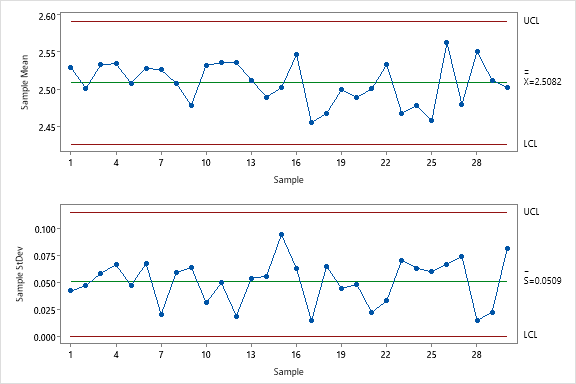
\includegraphics[width=0.5\textwidth]{Xbar_S_Paper.png}
\end{figure}


\item (14 pts) En una l\'inea de producci\'on de ejes para 
motores, el di\'ametro es una caracter\'istica crítica para el ensamblaje adecuado. 
Las especificaciones del di\'ametro son $50.00 \pm 0.50$ mm. Se mide el di\'ametro 
de un eje cada 30 minutos. Despu\'es de 15 horas de mediciones, se obtuvo el 
gr\'afico IMR con un promedio m\'ovil de orden 2 que se muestra abajo.
Calcula la probabilidad de que di\'ametro del eje se encuentre entre 49.7 mm y 
50.2 mm.
\begin{figure}[h!]
\centering
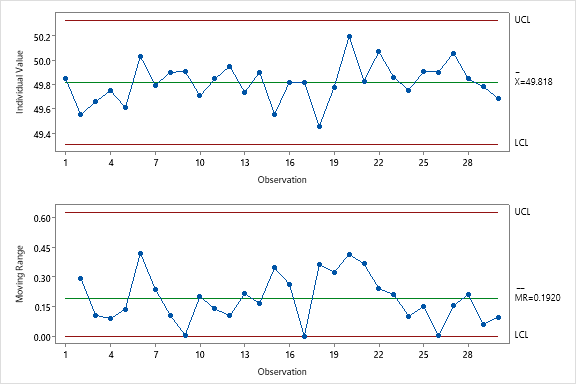
\includegraphics[width=0.5\textwidth]{IMR_Paper.png}
\end{figure}


\item (14 pts) Una m\'aquina de inyecci\'on de pl\'astico 
produce piezas de precisi\'on. Se ha determinado que la probabilidad de que una 
pieza tenga una rebaba fuera de tolerancia es de $0.05$. Durante una auditor\'a 
de calidad, un inspector toma una muestra aleatoria de $n = 16$ piezas de la 
l\'inea de producci\'on. ¿Cu\'al es la probabilidad de que el inspector 
encuentre exactamente 7 piezas defectuosas en esa muestra?

\item (14 pts) En una l\'inea de producci\'on de ejes para 
motores, el di\'ametro es una caracter\'istica crítica para el ensamblaje adecuado. 
Las especificaciones del di\'ametro son $50.00 \pm 0.40$ mm. Se mide el di\'ametro 
de un eje cada 30 minutos. Despu\'es de 15 horas de mediciones, se obtuvo el 
gr\'afico IMR con un promedio m\'ovil de orden 2 que se muestra abajo.
¿Es el proceso es capaz de cumplir con las especificaciones? Argumente.
\begin{figure}[h!]
\centering
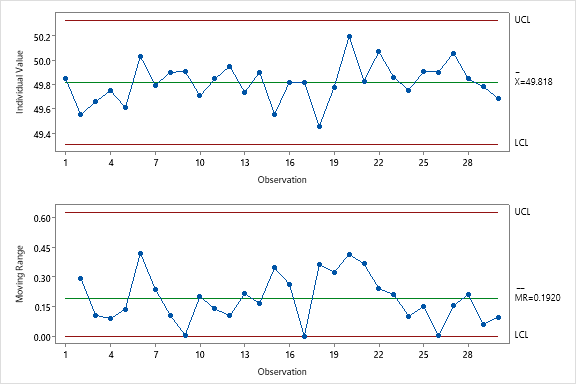
\includegraphics[width=0.5\textwidth]{IMR_Paper.png}
\end{figure}


\item (14 pts) Una empresa que fabrica tarjetas de circuitos 
impresos desea evaluar si la implementaci\'on de un nuevo sistema de ensamblaje 
ha reducido el n\'umero de disconformidades. Se tomaron 35 mediciones, antes y 
después del cambio, para analizar los efectos.
\begin{center}
\begin{tabular}{|l|c|c|}
\hline
 & Antes & Despu\'es \\ 
\hline
Media muestral & 3.60 & 3.21 \\ 
\hline
Desviaci\'on est\'andar muestral & 1.09 & 1.62 \\ 
\hline
\end{tabular}
\end{center}
Calcula un intervalo de confianza de 98\% para el número medio 
de disconformidades antes del cambio. Interprete su resultado.


\item (14 pts) Una empresa que fabrica l\'aminas de aluminio 
para la industria aeron\'autica necesita asegurar que el espesor de sus l\'aminas 
cumple con las especificaciones de $2.50 \pm 0.10$ mm. Se ha implementado una nueva 
maquinaria y se desea monitorear el espesor de las l\'aminas. Para ello, se han 
tomado muestras de tama\~no 5 cada hora y se gener\'o el diagrama que se muestra abajo.
Calcula los l\'imites de control para la {\bf variabilidad} del 
espesor de las láminas.
\begin{figure}[h!]
\centering
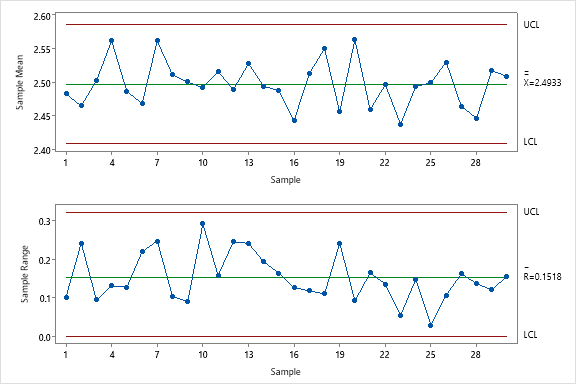
\includegraphics[width=0.5\textwidth]{Xbar_R_Paper.png}
\end{figure}


\item (14 pts) Una m\'aquina envasadora de detergente tiene 
una variabilidad natural con una desviaci\'on est\'andar de 8 ml, y la empresa 
debe garantizar que el 95.8\% de las botellas contengan al menos 500 ml para cumplir 
con la normativa de calidad. Determine a qu\'e valor promedio debe 
ajustarse la m\'aquina para que solo el 4.2\% de las botellas queden por debajo 
del contenido m\'inimo permitido.

\end{enumerate}

\newpage



\begin{center}
{An\'alisis Estad\'stico de Datos (Examen Argumentativo)}
\end{center}

Nombre: \underline{\hspace*{.2in}}
Héctor Gómez
\underline{\hspace*{.2in}} \quad Matr\'icula:\underline{\hspace*{.2in}}
A0000020
\underline{\hspace*{.2in}} \\

{\bf Instrucciones:} Muestra c\'omo obtienes tu respuesta. Puedes usar Excel 
o Minitab para tus cálculos de probabilidades o 
percentiles, pero no uses otros archivos o hagas uso de la IA. Respeta el 
c\'odigo de \'etica del curso y del Tecnol\'ogico 
de Monterrey.


\begin{enumerate}

\item (16 pts) Una empresa que fabrica l\'aminas de aluminio 
para la industria aeron\'autica necesita asegurar que el espesor de sus l\'aminas 
cumple con las especificaciones de $2.50 \pm 0.10$ mm. Se ha implementado una nueva 
maquinaria y se desea monitorear el espesor de las l\'aminas. Para ello, se han tomado 
muestras de tama\~no 5 cada hora y se gener\'o el diagrama que se muestra abajo.
Calcula los l\'imites de control para el espesor de las láminas.
\begin{figure}[h!]
\centering
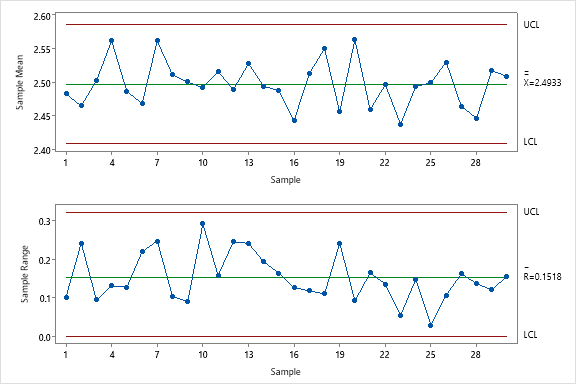
\includegraphics[width=0.5\textwidth]{Xbar_R_Paper.png}
\end{figure}


\item (14 pts) En una l\'inea de producci\'on de ejes para 
motores, el di\'ametro es una caracter\'istica crítica para el ensamblaje adecuado. 
Las especificaciones del di\'ametro son $50.00 \pm 0.50$ mm. Se mide el di\'ametro 
de un eje cada 30 minutos. Despu\'es de 15 horas de mediciones, se obtuvo el 
gr\'afico IMR con un promedio m\'ovil de orden 2 que se muestra abajo.
Calcula la probabilidad de que di\'ametro del eje se encuentre entre 49.9 mm y 
50.3 mm.
\begin{figure}[h!]
\centering
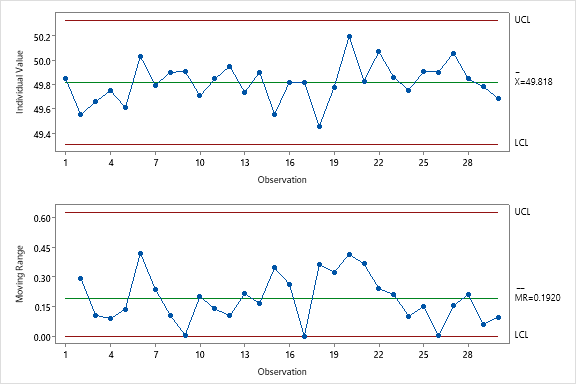
\includegraphics[width=0.5\textwidth]{IMR_Paper.png}
\end{figure}


\item (14 pts) Una m\'aquina de inyecci\'on de pl\'astico 
produce piezas de precisi\'on. Se ha determinado que la probabilidad de que una 
pieza tenga una rebaba fuera de tolerancia es de $0.05$. Durante una auditor\'a 
de calidad, un inspector toma una muestra aleatoria de $n = 16$ piezas de la 
l\'inea de producci\'on. ¿Cu\'al es la probabilidad de que el inspector 
encuentre exactamente 4 piezas defectuosas en esa muestra?

\item (14 pts) En una l\'inea de producci\'on de ejes para 
motores, el di\'ametro es una caracter\'istica crítica para el ensamblaje adecuado. 
Las especificaciones del di\'ametro son $50.00 \pm 0.50$ mm. Se mide el di\'ametro 
de un eje cada 30 minutos. Despu\'es de 15 horas de mediciones, se obtuvo el 
gr\'afico IMR con un promedio m\'ovil de orden 2 que se muestra abajo.
¿Es el proceso es capaz de cumplir con las especificaciones? Argumente.
\begin{figure}[h!]
\centering
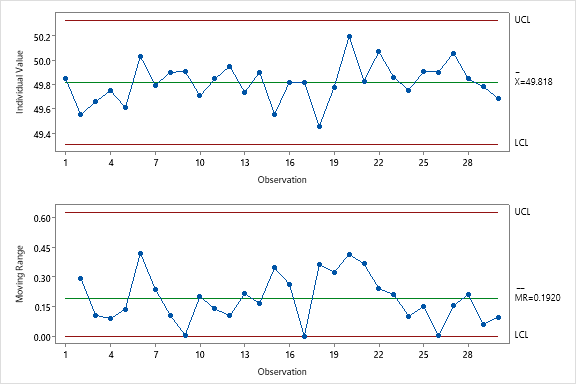
\includegraphics[width=0.5\textwidth]{IMR_Paper.png}
\end{figure}


\item (14 pts) Una empresa que fabrica tarjetas de circuitos 
impresos desea evaluar si la implementaci\'on de un nuevo sistema de ensamblaje 
ha reducido el n\'umero de disconformidades. Se tomaron 42 mediciones, antes y 
después del cambio, para analizar los efectos.
\begin{center}
\begin{tabular}{|l|c|c|}
\hline
 & Antes & Despu\'es \\ 
\hline
Media muestral & 3.60 & 2.64 \\ 
\hline
Desviaci\'on est\'andar muestral & 1.09 & 1.62 \\ 
\hline
\end{tabular}
\end{center}
Calcula un intervalo de confianza de 94\% para el número medio 
de disconformidades antes del cambio. Interprete su resultado.


\item (14 pts) Una empresa que fabrica l\'aminas de aluminio para 
la industria aeron\'autica necesita asegurar que el espesor de sus l\'aminas cumple 
con las especificaciones de $2.50 \pm 0.10$ mm. Se ha implementado una nueva maquinaria 
y se desea monitorear el espesor de las l\'aminas. Para ello, se han tomado muestras 
de tama\~no 4 cada hora y se gener\'o el diagrama que se muestra abajo.
Calcula los l\'imites de control para la {\bf variabilidad} del 
espesor de las láminas.
\begin{figure}[h!]
\centering
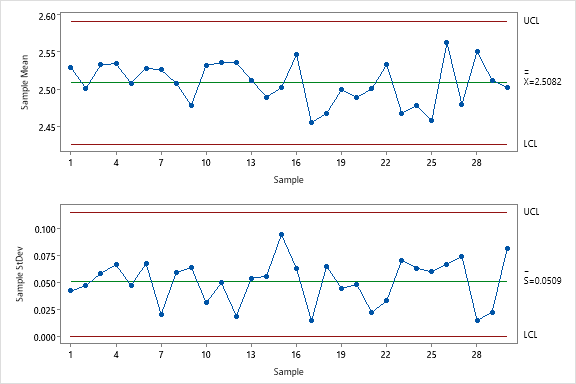
\includegraphics[width=0.5\textwidth]{Xbar_S_Paper.png}
\end{figure}


\item (14 pts) Una m\'aquina envasadora de detergente tiene 
una variabilidad natural con una desviaci\'on est\'andar de 8 ml, y la empresa 
debe garantizar que el 80.2\% de las botellas contengan al menos 500 ml para cumplir 
con la normativa de calidad. Determine a qu\'e valor promedio debe 
ajustarse la m\'aquina para que solo el 19.8\% de las botellas queden por debajo 
del contenido m\'inimo permitido.

\end{enumerate}

\newpage


\end{document}
